\documentclass[]{article}
\usepackage{lmodern}
\usepackage{amssymb,amsmath}
\usepackage{ifxetex,ifluatex}
\usepackage{fixltx2e} % provides \textsubscript
\ifnum 0\ifxetex 1\fi\ifluatex 1\fi=0 % if pdftex
  \usepackage[T1]{fontenc}
  \usepackage[utf8]{inputenc}
\else % if luatex or xelatex
  \ifxetex
    \usepackage{mathspec}
  \else
    \usepackage{fontspec}
  \fi
  \defaultfontfeatures{Ligatures=TeX,Scale=MatchLowercase}
\fi
% use upquote if available, for straight quotes in verbatim environments
\IfFileExists{upquote.sty}{\usepackage{upquote}}{}
% use microtype if available
\IfFileExists{microtype.sty}{%
\usepackage{microtype}
\UseMicrotypeSet[protrusion]{basicmath} % disable protrusion for tt fonts
}{}
\usepackage[margin=1in]{geometry}
\usepackage{hyperref}
\hypersetup{unicode=true,
            pdftitle={Supporting Information: The Regional Effects of Marine Protected Areas},
            pdfauthor={Daniel Ovando,Jennifer E. Caselle,Christopher Costello,Olivier Deschenes,Steven D. Gaines,Ray Hilborn,Owen Liu},
            pdfborder={0 0 0},
            breaklinks=true}
\urlstyle{same}  % don't use monospace font for urls
\usepackage{longtable,booktabs}
\usepackage{graphicx}
% grffile has become a legacy package: https://ctan.org/pkg/grffile
\IfFileExists{grffile.sty}{%
\usepackage{grffile}
}{}
\makeatletter
\def\maxwidth{\ifdim\Gin@nat@width>\linewidth\linewidth\else\Gin@nat@width\fi}
\def\maxheight{\ifdim\Gin@nat@height>\textheight\textheight\else\Gin@nat@height\fi}
\makeatother
% Scale images if necessary, so that they will not overflow the page
% margins by default, and it is still possible to overwrite the defaults
% using explicit options in \includegraphics[width, height, ...]{}
\setkeys{Gin}{width=\maxwidth,height=\maxheight,keepaspectratio}
\IfFileExists{parskip.sty}{%
\usepackage{parskip}
}{% else
\setlength{\parindent}{0pt}
\setlength{\parskip}{6pt plus 2pt minus 1pt}
}
\setlength{\emergencystretch}{3em}  % prevent overfull lines
\providecommand{\tightlist}{%
  \setlength{\itemsep}{0pt}\setlength{\parskip}{0pt}}
\setcounter{secnumdepth}{5}
% Redefines (sub)paragraphs to behave more like sections
\ifx\paragraph\undefined\else
\let\oldparagraph\paragraph
\renewcommand{\paragraph}[1]{\oldparagraph{#1}\mbox{}}
\fi
\ifx\subparagraph\undefined\else
\let\oldsubparagraph\subparagraph
\renewcommand{\subparagraph}[1]{\oldsubparagraph{#1}\mbox{}}
\fi

%%% Use protect on footnotes to avoid problems with footnotes in titles
\let\rmarkdownfootnote\footnote%
\def\footnote{\protect\rmarkdownfootnote}

%%% Change title format to be more compact
\usepackage{titling}

% Create subtitle command for use in maketitle
\providecommand{\subtitle}[1]{
  \posttitle{
    \begin{center}\large#1\end{center}
    }
}

\setlength{\droptitle}{-2em}

  \title{Supporting Information: The Regional Effects of Marine Protected Areas}
    \pretitle{\vspace{\droptitle}\centering\huge}
  \posttitle{\par}
    \author{Daniel Ovando,Jennifer E. Caselle,Christopher Costello,Olivier Deschenes,Steven D. Gaines,Ray Hilborn,Owen Liu}
    \preauthor{\centering\large\emph}
  \postauthor{\par}
    \date{}
    \predate{}\postdate{}
  
\usepackage{booktabs}
\usepackage{longtable}
\usepackage{array}
\usepackage{multirow}
\usepackage{wrapfig}
\usepackage{float}
\usepackage{colortbl}
\usepackage{pdflscape}
\usepackage{tabu}
\usepackage{threeparttable}
\usepackage{threeparttablex}
\usepackage[normalem]{ulem}
\usepackage{makecell}
\usepackage{xcolor}

\usepackage{longtable}
\usepackage{booktabs}
\usepackage{eso-pic}
\usepackage{graphicx}
\usepackage[left]{lineno}
\usepackage{xcolor}
\linenumbers

\begin{document}
\maketitle

{
\setcounter{tocdepth}{2}
\tableofcontents
}
\hypertarget{supporting-information-si}{%
\section{Supporting Information (SI)}\label{supporting-information-si}}

\hypertarget{si-text}{%
\section*{SI Text}\label{si-text}}
\addcontentsline{toc}{section}{SI Text}

\hypertarget{computing-environment}{%
\subsection{Computing environment}\label{computing-environment}}

All code needed to reproduce our main results and manuscript can be found at \url{https://github.com/DanOvando/regional-effects-of-mpas}. A fully reproducible environment for running this analysis and compiling the manuscript will be made available through Code Ocean at \url{https://codeocean.com/capsule/5233105/tree}. All analysis were performed in R version 3.6.1 (2019-07-05). Package versions are shown in Table.S\ref{tab:pkg-info}.

\begin{longtable}[t]{lllll}
\caption{\label{tab:pkg-info}Package versions and sources used in this paper}\\
\toprule
  & package & loadedversion & date & source\\
\midrule
\endfirsthead
\caption[]{\label{tab:pkg-info}Package versions and sources used in this paper \textit{(continued)}}\\
\toprule
  & package & loadedversion & date & source\\
\midrule
\endhead
\
\endfoot
\bottomrule
\endlastfoot
assertthat & assertthat & 0.2.1 & 2019-03-21 & CRAN (R 3.6.0)\\
backports & backports & 1.1.5 & 2019-10-02 & CRAN (R 3.6.1)\\
base64enc & base64enc & 0.1-3 & 2015-07-28 & CRAN (R 3.6.0)\\
bayesplot & bayesplot & 1.7.0 & 2019-05-23 & CRAN (R 3.6.0)\\
bitops & bitops & 1.0-6 & 2013-08-17 & CRAN (R 3.6.0)\\
\addlinespace
bookdown & bookdown & 0.15 & 2019-11-12 & CRAN (R 3.6.0)\\
boot & boot & 1.3-23 & 2019-07-05 & CRAN (R 3.6.0)\\
broom & broom & 0.5.2 & 2019-04-07 & CRAN (R 3.6.0)\\
callr & callr & 3.3.2 & 2019-09-22 & CRAN (R 3.6.0)\\
caret & caret & 6.0-84 & 2019-04-27 & CRAN (R 3.6.0)\\
\addlinespace
cellranger & cellranger & 1.1.0 & 2016-07-27 & CRAN (R 3.6.0)\\
class & class & 7.3-15 & 2019-01-01 & CRAN (R 3.6.1)\\
classInt & classInt & 0.4-2 & 2019-10-17 & CRAN (R 3.6.0)\\
cli & cli & 1.1.0 & 2019-03-19 & CRAN (R 3.6.0)\\
codetools & codetools & 0.2-16 & 2018-12-24 & CRAN (R 3.6.1)\\
\addlinespace
colorspace & colorspace & 1.4-1 & 2019-03-18 & CRAN (R 3.6.0)\\
colourpicker & colourpicker & 1.0 & 2017-09-27 & CRAN (R 3.6.0)\\
crayon & crayon & 1.3.4 & 2017-09-16 & CRAN (R 3.6.0)\\
crosstalk & crosstalk & 1.0.0 & 2016-12-21 & CRAN (R 3.6.0)\\
crul & crul & 0.9.0 & 2019-11-06 & CRAN (R 3.6.0)\\
\addlinespace
curl & curl & 4.2 & 2019-09-24 & CRAN (R 3.6.0)\\
data.table & data.table & 1.12.6 & 2019-10-18 & CRAN (R 3.6.0)\\
DBI & DBI & 1.0.0 & 2018-05-02 & CRAN (R 3.6.0)\\
desc & desc & 1.2.0 & 2018-05-01 & CRAN (R 3.6.0)\\
devtools & devtools & 2.2.1 & 2019-09-24 & CRAN (R 3.6.0)\\
\addlinespace
digest & digest & 0.6.23 & 2019-11-23 & CRAN (R 3.6.0)\\
doParallel & doParallel & 1.0.15 & 2019-08-02 & CRAN (R 3.6.0)\\
dplyr & dplyr & 0.8.3 & 2019-07-04 & CRAN (R 3.6.0)\\
DT & DT & 0.10 & 2019-11-12 & CRAN (R 3.6.0)\\
dygraphs & dygraphs & 1.1.1.6 & 2018-07-11 & CRAN (R 3.6.0)\\
\addlinespace
e1071 & e1071 & 1.7-2 & 2019-06-05 & CRAN (R 3.6.0)\\
ellipsis & ellipsis & 0.3.0 & 2019-09-20 & CRAN (R 3.6.0)\\
evaluate & evaluate & 0.14 & 2019-05-28 & CRAN (R 3.6.0)\\
extrafont & extrafont & 0.17 & 2014-12-08 & CRAN (R 3.6.0)\\
extrafontdb & extrafontdb & 1.0 & 2012-06-11 & CRAN (R 3.6.0)\\
\addlinespace
farver & farver & 2.0.1 & 2019-11-13 & CRAN (R 3.6.0)\\
fastmap & fastmap & 1.0.1 & 2019-10-08 & CRAN (R 3.6.0)\\
FishLife & FishLife & 2.0.0 & 2019-11-17 & Github (james-thorson/FishLife@3a6bdca)\\
forcats & forcats & 0.4.0 & 2019-02-17 & CRAN (R 3.6.0)\\
foreach & foreach & 1.4.7 & 2019-07-27 & CRAN (R 3.6.0)\\
\addlinespace
foreign & foreign & 0.8-72 & 2019-08-02 & CRAN (R 3.6.0)\\
fs & fs & 1.3.1 & 2019-05-06 & CRAN (R 3.6.0)\\
furrr & furrr & 0.1.0 & 2018-05-16 & CRAN (R 3.6.0)\\
future & future & 1.15.0 & 2019-11-08 & CRAN (R 3.6.0)\\
gdtools & gdtools & 0.2.1 & 2019-10-14 & CRAN (R 3.6.0)\\
\addlinespace
generics & generics & 0.0.2 & 2018-11-29 & CRAN (R 3.6.0)\\
geojson & geojson & 0.3.2 & 2019-01-31 & CRAN (R 3.6.0)\\
geojsonio & geojsonio & 0.8.0 & 2019-10-29 & CRAN (R 3.6.0)\\
geojsonlint & geojsonlint & 0.3.0 & 2019-02-08 & CRAN (R 3.6.0)\\
gganimate & gganimate & 1.0.4 & 2019-11-18 & CRAN (R 3.6.1)\\
\addlinespace
ggmap & ggmap & 3.0.0.901 & 2019-10-05 & Github (dkahle/ggmap@37a8672)\\
ggplot2 & ggplot2 & 3.2.1 & 2019-08-10 & CRAN (R 3.6.0)\\
ggridges & ggridges & 0.5.1 & 2018-09-27 & CRAN (R 3.6.0)\\
ggsci & ggsci & 2.9 & 2018-05-14 & CRAN (R 3.6.0)\\
ggspatial & ggspatial & 1.0.3 & 2018-12-14 & CRAN (R 3.6.0)\\
\addlinespace
gh & gh & 1.0.1 & 2017-07-16 & CRAN (R 3.6.0)\\
gifski & gifski & 0.8.6 & 2018-09-28 & CRAN (R 3.6.0)\\
globals & globals & 0.12.4 & 2018-10-11 & CRAN (R 3.6.0)\\
glue & glue & 1.3.1 & 2019-03-12 & CRAN (R 3.6.0)\\
gower & gower & 0.2.1 & 2019-05-14 & CRAN (R 3.6.0)\\
\addlinespace
gridExtra & gridExtra & 2.3 & 2017-09-09 & CRAN (R 3.6.0)\\
gtable & gtable & 0.3.0 & 2019-03-25 & CRAN (R 3.6.0)\\
gtools & gtools & 3.8.1 & 2018-06-26 & CRAN (R 3.6.0)\\
haven & haven & 2.2.0 & 2019-11-08 & CRAN (R 3.6.0)\\
here & here & 0.1 & 2017-05-28 & CRAN (R 3.6.0)\\
\addlinespace
hms & hms & 0.5.2 & 2019-10-30 & CRAN (R 3.6.0)\\
hrbrthemes & hrbrthemes & 0.6.0 & 2019-01-21 & CRAN (R 3.6.0)\\
htmltools & htmltools & 0.4.0 & 2019-10-04 & CRAN (R 3.6.1)\\
htmlwidgets & htmlwidgets & 1.5.1 & 2019-10-08 & CRAN (R 3.6.0)\\
httpcode & httpcode & 0.2.0 & 2016-11-14 & CRAN (R 3.6.0)\\
\addlinespace
httpuv & httpuv & 1.5.2 & 2019-09-11 & CRAN (R 3.6.0)\\
httr & httr & 1.4.1 & 2019-08-05 & CRAN (R 3.6.1)\\
igraph & igraph & 1.2.4.1 & 2019-04-22 & CRAN (R 3.6.0)\\
inline & inline & 0.3.15 & 2018-05-18 & CRAN (R 3.6.0)\\
ipred & ipred & 0.9-9 & 2019-04-28 & CRAN (R 3.6.0)\\
\addlinespace
iterators & iterators & 1.0.12 & 2019-07-26 & CRAN (R 3.6.0)\\
jpeg & jpeg & 0.1-8.1 & 2019-10-24 & CRAN (R 3.6.0)\\
jqr & jqr & 1.1.0 & 2018-10-22 & CRAN (R 3.6.0)\\
jsonlite & jsonlite & 1.6 & 2018-12-07 & CRAN (R 3.6.0)\\
jsonvalidate & jsonvalidate & 1.1.0 & 2019-06-25 & CRAN (R 3.6.0)\\
\addlinespace
kernlab & kernlab & 0.9-29 & 2019-11-12 & CRAN (R 3.6.0)\\
KernSmooth & KernSmooth & 2.23-16 & 2019-10-15 & CRAN (R 3.6.0)\\
knitr & knitr & 1.26 & 2019-11-12 & CRAN (R 3.6.0)\\
labeling & labeling & 0.3 & 2014-08-23 & CRAN (R 3.6.0)\\
later & later & 1.0.0 & 2019-10-04 & CRAN (R 3.6.1)\\
\addlinespace
lattice & lattice & 0.20-38 & 2018-11-04 & CRAN (R 3.6.1)\\
lava & lava & 1.6.6 & 2019-08-01 & CRAN (R 3.6.0)\\
lazyeval & lazyeval & 0.2.2 & 2019-03-15 & CRAN (R 3.6.0)\\
lifecycle & lifecycle & 0.1.0 & 2019-08-01 & CRAN (R 3.6.0)\\
listenv & listenv & 0.7.0 & 2018-01-21 & CRAN (R 3.6.0)\\
\addlinespace
lme4 & lme4 & 1.1-21 & 2019-03-05 & CRAN (R 3.6.0)\\
loo & loo & 2.1.0 & 2019-03-13 & CRAN (R 3.6.0)\\
lubridate & lubridate & 1.7.4 & 2018-04-11 & CRAN (R 3.6.0)\\
magrittr & magrittr & 1.5 & 2014-11-22 & CRAN (R 3.6.0)\\
maptools & maptools & 0.9-8 & 2019-10-05 & CRAN (R 3.6.0)\\
\addlinespace
markdown & markdown & 1.1 & 2019-08-07 & CRAN (R 3.6.0)\\
MASS & MASS & 7.3-51.4 & 2019-03-31 & CRAN (R 3.6.1)\\
Matrix & Matrix & 1.2-17 & 2019-03-22 & CRAN (R 3.6.1)\\
matrixStats & matrixStats & 0.55.0 & 2019-09-07 & CRAN (R 3.6.0)\\
memoise & memoise & 1.1.0 & 2017-04-21 & CRAN (R 3.6.0)\\
\addlinespace
mime & mime & 0.7 & 2019-06-11 & CRAN (R 3.6.0)\\
miniUI & miniUI & 0.1.1.1 & 2018-05-18 & CRAN (R 3.6.0)\\
minqa & minqa & 1.2.4 & 2014-10-09 & CRAN (R 3.6.0)\\
ModelMetrics & ModelMetrics & 1.2.2 & 2018-11-03 & CRAN (R 3.6.0)\\
modelr & modelr & 0.1.5 & 2019-08-08 & CRAN (R 3.6.0)\\
\addlinespace
munsell & munsell & 0.5.0 & 2018-06-12 & CRAN (R 3.6.0)\\
ncdf4 & ncdf4 & 1.17 & 2019-10-23 & CRAN (R 3.6.0)\\
nlme & nlme & 3.1-142 & 2019-11-07 & CRAN (R 3.6.0)\\
nloptr & nloptr & 1.2.1 & 2018-10-03 & CRAN (R 3.6.0)\\
nnet & nnet & 7.3-12 & 2016-02-02 & CRAN (R 3.6.1)\\
\addlinespace
numDeriv & numDeriv & 2016.8-1.1 & 2019-06-06 & CRAN (R 3.6.0)\\
optimx & optimx & 2018-7.10 & 2018-09-30 & CRAN (R 3.6.0)\\
packrat & packrat & 0.5.0 & 2018-11-14 & CRAN (R 3.6.0)\\
patchwork & patchwork & 1.0.0 & 2019-12-01 & CRAN (R 3.6.1)\\
pillar & pillar & 1.4.2 & 2019-06-29 & CRAN (R 3.6.0)\\
\addlinespace
pkgbuild & pkgbuild & 1.0.6 & 2019-10-09 & CRAN (R 3.6.0)\\
pkgconfig & pkgconfig & 2.0.3 & 2019-09-22 & CRAN (R 3.6.0)\\
pkgload & pkgload & 1.0.2 & 2018-10-29 & CRAN (R 3.6.0)\\
plotROC & plotROC & 2.2.1 & 2018-06-23 & CRAN (R 3.6.0)\\
plyr & plyr & 1.8.4 & 2016-06-08 & CRAN (R 3.6.0)\\
\addlinespace
png & png & 0.1-7 & 2013-12-03 & CRAN (R 3.6.0)\\
prettyunits & prettyunits & 1.0.2 & 2015-07-13 & CRAN (R 3.6.0)\\
processx & processx & 3.4.1 & 2019-07-18 & CRAN (R 3.6.0)\\
prodlim & prodlim & 2019.11.13 & 2019-11-17 & CRAN (R 3.6.1)\\
progress & progress & 1.2.2 & 2019-05-16 & CRAN (R 3.6.0)\\
\addlinespace
promises & promises & 1.1.0 & 2019-10-04 & CRAN (R 3.6.1)\\
ps & ps & 1.3.0 & 2018-12-21 & CRAN (R 3.6.0)\\
purrr & purrr & 0.3.3 & 2019-10-18 & CRAN (R 3.6.0)\\
R6 & R6 & 2.4.1 & 2019-11-12 & CRAN (R 3.6.0)\\
RANN & RANN & 2.6.1 & 2019-01-08 & CRAN (R 3.6.0)\\
\addlinespace
Rcpp & Rcpp & 1.0.3 & 2019-11-08 & CRAN (R 3.6.0)\\
RcppRoll & RcppRoll & 0.3.0 & 2018-06-05 & CRAN (R 3.6.0)\\
readr & readr & 1.3.1 & 2018-12-21 & CRAN (R 3.6.0)\\
readxl & readxl & 1.3.1 & 2019-03-13 & CRAN (R 3.6.0)\\
recipes & recipes & 0.1.7 & 2019-09-15 & CRAN (R 3.6.0)\\
\addlinespace
rEDM & rEDM & 0.7.4 & 2019-08-19 & Github (ha0ye/rEDM@88554a4)\\
remotes & remotes & 2.1.0 & 2019-06-24 & CRAN (R 3.6.0)\\
reshape2 & reshape2 & 1.4.3 & 2017-12-11 & CRAN (R 3.6.0)\\
rfishbase & rfishbase & 3.0.4 & 2019-06-27 & CRAN (R 3.6.0)\\
rgdal & rgdal & 1.4-7 & 2019-10-28 & CRAN (R 3.6.0)\\
\addlinespace
rgeos & rgeos & 0.5-2 & 2019-10-03 & CRAN (R 3.6.0)\\
RgoogleMaps & RgoogleMaps & 1.4.4 & 2019-08-20 & CRAN (R 3.6.0)\\
rjson & rjson & 0.2.20 & 2018-06-08 & CRAN (R 3.6.0)\\
rlang & rlang & 0.4.2 & 2019-11-23 & CRAN (R 3.6.0)\\
rmapshaper & rmapshaper & 0.4.1 & 2018-10-16 & CRAN (R 3.6.0)\\
\addlinespace
rmarkdown & rmarkdown & 1.17 & 2019-11-13 & CRAN (R 3.6.0)\\
rpart & rpart & 4.1-15 & 2019-04-12 & CRAN (R 3.6.1)\\
rprojroot & rprojroot & 1.3-2 & 2018-01-03 & CRAN (R 3.6.0)\\
rsconnect & rsconnect & 0.8.15 & 2019-07-22 & CRAN (R 3.6.0)\\
rstan & rstan & 2.19.2 & 2019-07-09 & CRAN (R 3.6.0)\\
\addlinespace
rstanarm & rstanarm & 2.19.2 & 2019-10-03 & CRAN (R 3.6.1)\\
rstantools & rstantools & 2.0.0 & 2019-09-15 & CRAN (R 3.6.0)\\
rstudioapi & rstudioapi & 0.10 & 2019-03-19 & CRAN (R 3.6.0)\\
rticles & rticles & 0.12 & 2019-11-12 & CRAN (R 3.6.0)\\
Rttf2pt1 & Rttf2pt1 & 1.3.7 & 2018-06-29 & CRAN (R 3.6.0)\\
\addlinespace
rvest & rvest & 0.3.5 & 2019-11-08 & CRAN (R 3.6.0)\\
scales & scales & 1.1.0 & 2019-11-18 & CRAN (R 3.6.0)\\
sessioninfo & sessioninfo & 1.1.1 & 2018-11-05 & CRAN (R 3.6.0)\\
sf & sf & 0.8-0 & 2019-09-17 & CRAN (R 3.6.1)\\
shiny & shiny & 1.4.0 & 2019-10-10 & CRAN (R 3.6.0)\\
\addlinespace
shinyjs & shinyjs & 1.0 & 2018-01-08 & CRAN (R 3.6.0)\\
shinystan & shinystan & 2.5.0 & 2018-05-01 & CRAN (R 3.6.0)\\
shinythemes & shinythemes & 1.1.2 & 2018-11-06 & CRAN (R 3.6.0)\\
sp & sp & 1.3-2 & 2019-11-07 & CRAN (R 3.6.0)\\
spasm & spasm & 0.1.0.9000 & 2019-10-16 & local\\
\addlinespace
StanHeaders & StanHeaders & 2.19.0 & 2019-09-07 & CRAN (R 3.6.0)\\
stringi & stringi & 1.4.3 & 2019-03-12 & CRAN (R 3.6.0)\\
stringr & stringr & 1.4.0 & 2019-02-10 & CRAN (R 3.6.0)\\
survival & survival & 3.1-7 & 2019-11-09 & CRAN (R 3.6.0)\\
Synth & Synth & 1.1-5 & 2014-01-27 & CRAN (R 3.6.0)\\
\addlinespace
systemfonts & systemfonts & 0.1.1 & 2019-07-01 & CRAN (R 3.6.0)\\
testthat & testthat & 2.3.0 & 2019-11-05 & CRAN (R 3.6.0)\\
threejs & threejs & 0.3.1 & 2017-08-13 & CRAN (R 3.6.0)\\
tibble & tibble & 2.1.3 & 2019-06-06 & CRAN (R 3.6.0)\\
tidyr & tidyr & 1.0.0 & 2019-09-11 & CRAN (R 3.6.0)\\
\addlinespace
tidyselect & tidyselect & 0.2.5 & 2018-10-11 & CRAN (R 3.6.0)\\
tidyverse & tidyverse & 1.2.1 & 2017-11-14 & CRAN (R 3.6.0)\\
timeDate & timeDate & 3043.102 & 2018-02-21 & CRAN (R 3.6.0)\\
tinytex & tinytex & 0.17 & 2019-10-30 & CRAN (R 3.6.0)\\
TMB & TMB & 1.7.15 & 2018-11-09 & CRAN (R 3.6.0)\\
\addlinespace
tweenr & tweenr & 1.0.1 & 2018-12-14 & CRAN (R 3.6.0)\\
units & units & 0.6-5 & 2019-10-08 & CRAN (R 3.6.0)\\
usethis & usethis & 1.5.1 & 2019-07-04 & CRAN (R 3.6.0)\\
V8 & V8 & 2.3 & 2019-07-02 & CRAN (R 3.6.0)\\
vctrs & vctrs & 0.2.0 & 2019-07-05 & CRAN (R 3.6.0)\\
\addlinespace
viridis & viridis & 0.5.1 & 2018-03-29 & CRAN (R 3.6.0)\\
viridisLite & viridisLite & 0.3.0 & 2018-02-01 & CRAN (R 3.6.0)\\
withr & withr & 2.1.2 & 2018-03-15 & CRAN (R 3.6.0)\\
xfun & xfun & 0.11 & 2019-11-12 & CRAN (R 3.6.0)\\
xml2 & xml2 & 1.2.2 & 2019-08-09 & CRAN (R 3.6.0)\\
\addlinespace
xtable & xtable & 1.8-4 & 2019-04-21 & CRAN (R 3.6.0)\\
xts & xts & 0.11-2 & 2018-11-05 & CRAN (R 3.6.0)\\
yaml & yaml & 2.2.0 & 2018-07-25 & CRAN (R 3.6.0)\\
zeallot & zeallot & 0.1.0 & 2018-01-28 & CRAN (R 3.6.0)\\
zoo & zoo & 1.8-6 & 2019-05-28 & CRAN (R 3.6.0)\\*
\end{longtable}

\hypertarget{operating-model}{%
\subsection{Operating Model}\label{operating-model}}

The operating model is a spatial single-species age-structured bio-economic model. The operating model itself is organized as an R package, which can be found and installed at \url{https://github.com/DanOvando/spasm}. Users can explore the functionality of the operating mode through an interactive web application at \url{https://danovando.shinyapps.io/simmpa/}.

For the population model, numbers \emph{n} at time \emph{t} for age \emph{a} are given by

\begin{equation}
n_{t,a}=\begin{cases}
      = BH(ssb_{t-1}) & \text{if $a = 1$}\\
     = n_{t-1,a-1}e^{-(m + qE_{t-1}{\times}s_{a-1})}, & \text{if $1< a < max(age)$}\\
     =  n_{t-1,a}e^{-(m + qE_{t-1}{\times}s_a)} + n_{t-1,a-1}e^{-(m + qE_{t-1}{\times}s_{a-1})}, & \text{if $a = max(a)$}
  \end{cases}
  \label{eq:pop}
\end{equation}

where \emph{BH} is the Beverton-Holt recruitment function, \emph{ssb} is spawning-stock-biomass, \emph{m} is natural mortality, \emph{q} is catchability,\emph{E} is fishing effort at time \emph{t}, and \emph{s} is selectivity at age \emph{a}.

Selectivity is modeled through a logistic form per

\begin{equation}
s_a=\frac{1}{(1 + e^{-log(19)\times\frac{l_a - l_{sel}}{\delta_{sel}}})}
  \label{eq:sel}
\end{equation}

where \(l_a\) is the mean length at at age, \(l_sel\) is the length at which on average 50\% of individuals are selected by the fishery, and \(\delta_{sel}\) are the additional units of length at which on average 95\% of fish are selected by the fishery.

\emph{ssb} is calculated by converting age to mean length, calculating weight at age, maturity at age, and then calculating spawning stock biomass as the sum of spawning potential at age in a given time step.

\begin{equation}
  l_{a} = l_{\infty}\left(1 - e^{-k(a - a_0)}\right)
  \label{eq:len}
\end{equation}

Weight at age is then given by

\begin{equation}
  b_{a} = w_a \times l_{a}^{w_b}
  \label{eq:weight}
\end{equation}

and maturity \emph{mat} is calculated as

\begin{equation}
  \frac{1}{(1 + e^{-log(19)\times\frac{l_a - l_{mat}}{\delta_{mat}}})}
  \label{eq:mat}
\end{equation}

where \(l_{mat}\) is the length at which on average 50\% of individuals are sexual maturity, and \(\delta_{mat}\) is the units of length beyond \(l_{mat}\) at which on average 95\% of fish are sexually mature.

Spawning stock biomass at time \emph{t} is then calculated as

\begin{equation}
  ssb_t = \sum_{a=1}^Aw_{a,t}mat_{a,t}n_{a,t}
    \label{eq:ssb}
\end{equation}

\hypertarget{recruitment}{%
\subsubsection{Recruitment}\label{recruitment}}

Recruitment follows Beverton-Holt dynamics. We do however allow for three variants in the timing of density dependence:

\begin{enumerate}
\def\labelenumi{\arabic{enumi}.}
\tightlist
\item
  Local density dependence: Density dependence occurs independently in each patch, and recruits then disperse to nearby patches
\end{enumerate}

\begin{equation}
  n_{t,a = 1,p} = \left(\frac{0.8{\times}r0_{p}\times{h}\times{ssb_{t-1,p}}}{0.2\times{ssb0_p}\times(1 - h)+(h - 0.2)\times{ssb_{t-1,p}}}\right)\times \boldsymbol{d^l} \times \epsilon_t
  \label{eq:dd1}
\end{equation}

where \textbf{d\textsuperscript{l}} is the larval movement matrix, \emph{h} is Beverton-Holt steepness (constrained between 0.6 and 0.99), \emph{r0} is unfished recruitment, and \emph{ssb0} is unfished spawning stock biomass.

\begin{enumerate}
\def\labelenumi{\arabic{enumi}.}
\setcounter{enumi}{1}
\tightlist
\item
  Global density dependence: Density dependence is a function of the sum of spawning biomass across all patches, and recruits are then distributed according to habitat quality
\end{enumerate}

\begin{equation}
n_{t,a = 1,p} = \left(\frac{0.8{\times}\sum_{p=1}^P{r0_{p}}\times{h}\times\sum_{p=1}^P{ssb_{t-1,p}}}{0.2\times{\sum_{p=1}^Pssb0_p}\times(1 - h)+(h - 0.2)\times{\sum_{p=1}^Pssb_{t-1,p}}}\right)\times {hab_p} \times \epsilon_t
  \label{eq:dd2}
\end{equation}

where \emph{hab} is a vector of habitat quality by patch that sums to 1.

\begin{enumerate}
\def\labelenumi{\arabic{enumi}.}
\setcounter{enumi}{2}
\tightlist
\item
  Post-dispersal density dependence: Larvae are distributed throughout the system, and then density dependence occurs based on the density of adult biomass at the destination patch.
\end{enumerate}

\begin{equation}
  larv_{t,p} = ssb_{t-1} \times\boldsymbol{d^l}
  \label{eq:larvmove}
\end{equation}

\begin{equation}
n_{t,a = 1,p} = \left(\frac{0.8{\times}r0_{p}\times{h}\times{larv_{t,p}}}{0.2\times{ssb0_p}\times(1 - h)+(h - 0.2)\times{larv_{t,p}}}\right) \times \epsilon_t
  \label{eq:dd3}
\end{equation}

\(\epsilon\) represents multiplicative recruitment deviates. Deviates are calculated as

\[\epsilon_t = e^{recdev_t}\]

`\(recdev\) are the log-normal recruitment deviates in time \emph{t}.

The stochastic component of the deviate is

\[\gamma_t \sim norm(-\sigma_r^2/2,\sigma_r)\]

and the final multiplicative recruitment deviate in time \emph{t} is then

\[recdev_t = \gamma_t\sqrt{1 - ac_r^2} + recdev_{t-1}ac_r \]

where \emph{ac} is the autocorrelation of the recruitment function (between 0 and 1).

\hypertarget{dispersal}{%
\subsubsection{Dispersal}\label{dispersal}}

Dispersal in the model is broken into two components: adult and larval. Both assume a Gaussian dispersal kernel of the form

\begin{equation}
m_{s,p_i,p_j}=\frac{1}{\sqrt{2\pi\sigma_{s,p_i}^2}}e^{-\frac{d_{p_i,p_j}^2}{2\sigma_{s,p_i}^2}}
  \label{eq:move}
\end{equation}

where \emph{i} is the source patch, \emph{j} is the destination patch, \emph{d} is the distance between patches \emph{i} and \emph{j} (where distance is measured with wrapped edges, such that if there are 50 patches, patch 1 and patch 50 have a distance of 1), and \(\sigma_s*\)is the movement rate, in units of patches, for life stage \emph{s} (adult or larval).

We allow the adult dispersal matrix to be affected by adult density dependence. The idea behind this is that adult fish will move more as densities increase, and become more sedentary as densities decrease (as habitat and food become more available for example). This allows us to simulate a scenario where as MPAs build up density they begin to export more adults to the surrounding waters, and if densities are lower in the fished areas these fish will actually become more sedentary.

Under these conditions, the adult movement rate is a linear function of depletion (measured as \(ssb/ssb_0\))

\begin{equation}
\sigma_{s=a,p}^* = max(slope\times{d _p+ \sigma_{s=a} \times dmod},0)
  \label{eq:ddmove1}
\end{equation}

where

\begin{equation}
slope = \sigma_{s=a} - ( \sigma_{s=a} \times dmod)
  \label{eq:ddmove2}
\end{equation}

Under these conditions, when depletion \emph{d = 1} (meaning the stock is unfished) the adult movement rate equals the max adult movement rate (\(\sigma_{s=a}^* = \sigma_{s=a}\)). When \(d=0\) \(\sigma_{s=a}^* = \sigma_{s=a} * dmod\). The greater \emph{dmod} is then, the more movement rates from a patch decline as density declines.

We also allow for a ``sprinkler'' condition in which MPAs are placed in locations that disperse larvae to a much wider area than non-MPA locations. In this world, we simply multiply \(\sigma_{s=l,p}\) by a sprinkler factor (by default 4) for any patch \emph{p} that would eventually become an MPA (whether or not MPAs are ever introduced). In other words, when we compare two scenarios, one with MPA and one without, the ``without'' scenario still has higher larval movement rates in patches that become MPAs in the ``with'' scenario.

\hypertarget{fleet-dynamics}{%
\subsubsection{Fleet Dynamics}\label{fleet-dynamics}}

We allow for three fleet models: constant effort, constant catch, and open-access. Constant effort means that total effort across all patches is equal in all time steps (unless MPAs force exit of effort as discussed below). Under constant catch, we set a target catch volume (in biomass, summed across all patches). Each time step, we calculate the fishing mortality rate that, given the fishable biomass in that time step, would produce the target catch. If there is insufficient fishable biomass available to support the target catch, we mark the population as crashed and stop the simulation (these crashed simulations are not included in the final analysis).

Under open-access, fishing effort expands in proportion to a weighted mean of profit-per-unit effort over the last \emph{t} time steps.

\begin{equation}
profit_{t} = price\times{catch_t} - cost\times{E_t}^2
  \label{eq:profit}
\end{equation}

From there, we determine the new effort as

\begin{equation}
E_t = E_{t-1} + \theta\times\sum_{i=t-1-l}^{t-1}w_i\frac{profit_{i}}{E^i}
  \label{eq:openaccess}
\end{equation}

where \emph{w} is a weighting function which is just a linear function of time

\begin{equation}
  w_i = \frac{i}{\sum_{i=1}^li}
  \label{eq:oaweight}
\end{equation}

and \emph{l} is the number of lagged time steps over which to calculate the weighted mean PPUE.

The open-access model can enter chaotic dynamics if the model parameters are not properly tuned. To address this, we first set price at 1, and set a \(\theta\) such that when profits are about as large as they might conceivably be the fishery doubles in size. We then estimate reference points for the simulated fishery (Bmsy, Fmsy, MSY), and set a target bionomic equilibrium B/Bmsy. Holding the other parameters constant, we thing find a cost coefficient that produces the desired bionomic equilibrium.

\hypertarget{spatial-fleet-distribution}{%
\subsubsection{Spatial Fleet Distribution}\label{spatial-fleet-distribution}}

Given a total amount of effort, we then need to distribute that effort in space. In the simplest form, effort is evenly distributed throughout the available patches.

\begin{equation}
E_{t,p} = E_t \times \frac{open_p}{\sum_{p=1}^Popen_p}
  \label{eq:simpleeffort}
\end{equation}

where \emph{open} indicates whether patch \emph{p} is open to fishing or not.

Effort can also be distributed according to spawning stock biomass in fishable patches

\begin{equation}
E_{t,p} = E_t \times \frac{open_{t,p}ssb_{t,p}}{\sum_{p=1}^Popen_{t,p}ssb_{t,p}}
  \label{eq:biomasseffort}
\end{equation}

And lastly effort can be distributed according to profit-per-unit-effort

\begin{equation}
E_{t,p} = E_t \times \frac{open_{t,p}ppue_{t,p}}{\sum_{p=1}^Popen_{t,p}ppue_{t,p}}
  \label{eq:ppueeffort}
\end{equation}

Under the constant effort or open access scenarios, effort can immediately respond to MPA placement in one of two ways. Effort can concentrate outside the MPAs (such that the sum of effort before and after MPA placement stays constant), or effort can leave the MPAs, such that the total effort in the fishery is reduced by the amount of effort that occurred inside the MPAs immediately before MPA placement. This is intended to simulate a scenario where fishers that used to use the MPA simply leave the fishery rather than redistribute outside the MPA, due for example to costs or lack of location specific knowledge to fish outside the MPA.

\hypertarget{mpa-design}{%
\subsubsection{MPA Design}\label{mpa-design}}

MPA design is relatively straightforward. We set a percentage of patches that are to be placed inside no-take MPAs. MPAs can either be placed continuously (e.g if there are 100 patches and 25\% are in MPAs, patches 1 to 25 are in MPAs) or randomly. If the MPAs are placed randomly, we can also set a minimum MPA size. This controls the patchiness of the MPAs. As the ``patchiness'' factor approaches zero, the behavior equals that of random placement. As it approaches 1, the behavior approaches that of continuous placement. In between, the greater the patchiness, the more clustered together MPAs become.

\hypertarget{simulations}{%
\subsection{Simulations}\label{simulations}}

We use this our operating model to simulate 10,000 different fisheries, where each fishery is a random combination of variables, described below

Table.S1 - Range of simulated variables

\begin{longtable}[]{@{}rc@{}}
\toprule
\begin{minipage}[b]{0.41\columnwidth}\raggedleft
Variable\strut
\end{minipage} & \begin{minipage}[b]{0.53\columnwidth}\centering
Distribution\strut
\end{minipage}\tabularnewline
\midrule
\endhead
\begin{minipage}[t]{0.41\columnwidth}\raggedleft
Scientific Name\strut
\end{minipage} & \begin{minipage}[t]{0.53\columnwidth}\centering
Drawn from all possible species in \texttt{FishLife} (Thorson et al. (2017))\strut
\end{minipage}\tabularnewline
\begin{minipage}[t]{0.41\columnwidth}\raggedleft
steepness (h)\strut
\end{minipage} & \begin{minipage}[t]{0.53\columnwidth}\centering
\textasciitilde uniform(0.6,0.95)\strut
\end{minipage}\tabularnewline
\begin{minipage}[t]{0.41\columnwidth}\raggedleft
Adult movement (\(\sigma_{s=a}\))\strut
\end{minipage} & \begin{minipage}[t]{0.53\columnwidth}\centering
\textasciitilde uniform(0,0.5 * P)\strut
\end{minipage}\tabularnewline
\begin{minipage}[t]{0.41\columnwidth}\raggedleft
Larval movement (\(\sigma_{s=l}\))\strut
\end{minipage} & \begin{minipage}[t]{0.53\columnwidth}\centering
\textasciitilde uniform(0,0.5 * P)\strut
\end{minipage}\tabularnewline
\begin{minipage}[t]{0.41\columnwidth}\raggedleft
Recruitment variation (\(\sigma_{r}\))\strut
\end{minipage} & \begin{minipage}[t]{0.53\columnwidth}\centering
\(\in\{0,0.05,.1\}\)\strut
\end{minipage}\tabularnewline
\begin{minipage}[t]{0.41\columnwidth}\raggedleft
Recruitment autocorrelation (\(ac_{r}\))\strut
\end{minipage} & \begin{minipage}[t]{0.53\columnwidth}\centering
\(\in\{0,0.05,.1\}\)\strut
\end{minipage}\tabularnewline
\begin{minipage}[t]{0.41\columnwidth}\raggedleft
DD adult movement (dmod)\strut
\end{minipage} & \begin{minipage}[t]{0.53\columnwidth}\centering
\(\in\{0.25,1\}\)\strut
\end{minipage}\tabularnewline
\begin{minipage}[t]{0.41\columnwidth}\raggedleft
Density-dependence timing\strut
\end{minipage} & \begin{minipage}[t]{0.53\columnwidth}\centering
\(\in\{local, global,post-dispersal\}\)\strut
\end{minipage}\tabularnewline
\begin{minipage}[t]{0.41\columnwidth}\raggedleft
\% Patches in MPA\strut
\end{minipage} & \begin{minipage}[t]{0.53\columnwidth}\centering
\textasciitilde uniform(0.01,1)\strut
\end{minipage}\tabularnewline
\begin{minipage}[t]{0.41\columnwidth}\raggedleft
Initial fishing relative to natural mortality\strut
\end{minipage} & \begin{minipage}[t]{0.53\columnwidth}\centering
\textasciitilde uniform(0.01,4)\strut
\end{minipage}\tabularnewline
\begin{minipage}[t]{0.41\columnwidth}\raggedleft
Selectivity as a multiple of maturity length\strut
\end{minipage} & \begin{minipage}[t]{0.53\columnwidth}\centering
\textasciitilde uniform(0.1,1.25)\strut
\end{minipage}\tabularnewline
\begin{minipage}[t]{0.41\columnwidth}\raggedleft
Fleet model\strut
\end{minipage} & \begin{minipage}[t]{0.53\columnwidth}\centering
\(\in\{open-access, constant-effort,constant-catch\}\)\strut
\end{minipage}\tabularnewline
\begin{minipage}[t]{0.41\columnwidth}\raggedleft
Spatial effort model\strut
\end{minipage} & \begin{minipage}[t]{0.53\columnwidth}\centering
\(\in\{uniform, biomass,profits\}\)\strut
\end{minipage}\tabularnewline
\begin{minipage}[t]{0.41\columnwidth}\raggedleft
Years into simulation to start MPA\strut
\end{minipage} & \begin{minipage}[t]{0.53\columnwidth}\centering
\textasciitilde round(uniform(5,0.66 * T))\strut
\end{minipage}\tabularnewline
\begin{minipage}[t]{0.41\columnwidth}\raggedleft
MPA is sprinkler?\strut
\end{minipage} & \begin{minipage}[t]{0.53\columnwidth}\centering
\(\in\{TRUE,FALSE\}\)\strut
\end{minipage}\tabularnewline
\begin{minipage}[t]{0.41\columnwidth}\raggedleft
Randomly place MPA?\strut
\end{minipage} & \begin{minipage}[t]{0.53\columnwidth}\centering
\(\in\{TRUE,FALSE\}\)\strut
\end{minipage}\tabularnewline
\begin{minipage}[t]{0.41\columnwidth}\raggedleft
Fleet reaction to MPA\strut
\end{minipage} & \begin{minipage}[t]{0.53\columnwidth}\centering
\(\in\{concentrate, abandon-ship\}\)\strut
\end{minipage}\tabularnewline
\begin{minipage}[t]{0.41\columnwidth}\raggedleft
Patchiness\strut
\end{minipage} & \begin{minipage}[t]{0.53\columnwidth}\centering
\textasciitilde uniform(0.01,0.75)\strut
\end{minipage}\tabularnewline
\begin{minipage}[t]{0.41\columnwidth}\raggedleft
MPA habitat factor\strut
\end{minipage} & \begin{minipage}[t]{0.53\columnwidth}\centering
\(\in\{1, 4\}\)\strut
\end{minipage}\tabularnewline
\bottomrule
\end{longtable}

One thing to note here is the random sampling of species' scientific names. The effect of MPAs, especially over the short term, will clearly be affected by factors such as the growth rate, the mortality rate, and the maturity schedule. These life history traits are related through a variety of biological processes, as such randomly sampling these parameters can lead to biologically nonsensical ``frankenfish''. We resolve this by using the \texttt{FishLife} package (Thorson et al. (2017)) instead. \texttt{FishLife} builds off of \href{https://fishbase.org/}{FishBase}, and provides estimate of key life history traits taking into account the relationships across these variables. For simulations then, we randomly pull a species from \texttt{FishLife}, and then pull the available life history information from that species for use in the operating model. This allows us to simulate a wide range of life history types in a realistic manner.

We ran 20,000 simulations from these distributions. Each simulation runs for 50 years in 50 patches (with a 25 year unfished burn-in period for conditions in which initial conditions cannot be solved analytically, for example when MPAs have better habitat than non-MPAs). For each simulation, we run one scenario without MPAs, though taking note of where the MPA would be as needed. For the second scenario, we hold everything constant except we now add in the MPAs as dictated by the particular simulation.

\hypertarget{filtering-simulations}{%
\subparagraph{Filtering Simulations}\label{filtering-simulations}}

After the 20,000 simulations have run, we perform a series of filtering steps to remove runs that either a) produced chaotic dynamics during the open-access scenario; b) did not converge to the correct bionomic equilibrium in the open-access scenario; or c) crashed the population before the MPAs went into place (population falls below 5\% of unfished biomass). These filtering steps left us with 9672 viable simulations.

\hypertarget{additional-simulation-results}{%
\paragraph{Additional Simulation Results}\label{additional-simulation-results}}

Simulation results are presented as percent differences in biomass densities with and without MPAs, in order to be comparable to the estimates that the regression model produces. However, this metric presents some problems as a measure of how ``detectable'' an effect size is. As depletion increases, relatively small changes in total biomass (relative to the variance in the observation process) can translate into large percent changes in biomass. For example, moving from a density of .2kg/m\textsuperscript{2} to .4kg/m\textsuperscript{2} translates to a 100\% percent increase, but only a .2kg/m\textsuperscript{2} absolute increase, a small value to detect with a real observation program.

To illustrate these, we present an alternative to our simulation results in which changes in biomass caused by MPAs is scaled by the unfished biomass in the system.

\begin{figure}
\centering
\includegraphics{ovando-regional-effects-of-mpas-si_files/figure-latex/pop-conservation-effect-1.pdf}
\caption{\label{fig:pop-conservation-effect}Median (A) and range (B) of equilibrium regional MPA conservation effects (change in total biomass with MPAs relative to without MPAs as a percentage of unfished biomass) across a range of depletion and MPA sizes (and incorporating the full range of scenarios included in our study). `Range in MPA' is the percent of patches covered by an MPA, `Depletion' is the depletion that would have occurred in equilibrium without the MPA}
\end{figure}

\hypertarget{estimation-model}{%
\subsection{Estimation Model}\label{estimation-model}}

The goal of the estimation model is to estimate the difference in the mean densities of targeted and non-targeted species pre-and-post MPA implementation.

At the rawest level, the data are counts of finfish in 2cm length bins along a 30m x 2m transect at various sites and depths. These length bins are converted to biomass, and then biomass densities, by converting length to weights using available allometric data and dividing by the transect area. Our goal is to estimate the effect of the MPAs on these biomass densities of fish throughout the Channel Islands. We fit this model using a hierarchical mixed-effect framework using Template Model Builder (TMB, Kristensen et al. 2016) in R. The model consists of three levels, the first (starting from the ``bottom'') being transect-level densities of fish species observed by PISCO, which are standardized into a standardized biomass abundance index, accounting for both probability of detection and expected density as a result of changes in both abundance and covariates such as visibility and observer experience (see Maunder and Langley 2004). For the second stage, we break the abundance indices into targeted and non-targeted species (per the classifications in the PISCO data), and estimate the mean trend of each group (targeted and non-targeted) over time. In the third stage, we estimate the difference in the de-meaned trend between the targeted and non-targeted fishes (controlling for factors such as water temperature, kelp cover, and commercial fishery catches), that under the assumptions of the model reflects the causal effect of the MPAs on the outcome of interest (in this case regional biomass density of targeted fishes). All three of these steps are integrated into the same estimation model, in order to propagate uncertainty through the model correctly. Simpler versions of the estimation model, as well as a synthetic control identification strategy, were assessed as well and showed results consistent with the model in our main results.

\hypertarget{data}{%
\subsubsection{Data}\label{data}}

All observation data used in the estimation model were collected by PISCO. PISCO staff also compiled allometric information used to convert lengths to expected weights, and hence biomass densities. We do not account for error in this translation step Table.S\ref{tab:classcode} lists the species included in the model. In order to be included in the estimation model, a species must have been observed at least twice a year every year for at least 14 years. We also omitted all observations of ``young of the year'' fish due to inability to identify these observations to the nearest species level in many cases. We omitted data from 1999 due to changes in the sampling procedures that occurred after 1999. Per recommendations from PISCO staff we omit observations from the canopy level of the transects (leaving the middle, bottom, and middle canopy levels).

PISCO data report positive observations of fish. In order to use these data in our model we need to add in zeros for any transect that could have observed a given species of fish but did not. We assume that a fish could have been observed on a given transect if that species has ever been observed at that site in any time period in the data (PISCO data are organized by sites, with multiple transect at different locations within the borders of a site). If a species has never been observed at a site we assume that it does not occur at that site.

Interested readers can examine the mean biomass densities of all species in Fig.\ref{fig:targ-trend-plot}-\ref{fig:nontarg-trend-plot}.

We include several additional sources of data in our regression analysis. Temperature readings are included from the PISCO data for each transect. We also include PISCO data on the estimated surge and visibility. We augmented these data with information on kelp cover over time from the Santa Barbara Channel Long Term Ecological Research Network (LTER et al. 2017). We used a k-nearest neighbors algorithm to fill in missing kelp observations, and matched the interpolated kelp data to the PISCO data at the resolution of year-month-site (Fig.\ref{fig:kelp-plot}).

Temperature data were augmented with data from \texttt{FishLife} (Thorson et al. 2017) to include the estimated preferred temperature for a given species, so that we can include deviations from the preferred temperature envelope as a predictor in the model. This allows different temperatures to have different effects on each species (and is less computationally intensive than estimating species-temperature slopes) (Fig.\ref{fig:tempdev-plot}).

We also included lagged catch totals in the Santa Barbara region for the commercially harvest species in the database, in an effort to control for changes in density caused by changes in fishing pressure. Catches were pulled from the CDFW website (\url{https://www.wildlife.ca.gov/Fishing/Commercial/Landings}), and extracted using the \texttt{tabulizer} package in R (Leeper 2018) (Fig.\ref{fig:catches-plot}).

\begin{figure}
\centering
\includegraphics{ovando-regional-effects-of-mpas-si_files/figure-latex/tempdev-plot-1.pdf}
\caption{\label{fig:tempdev-plot}Mean deviations from preferred temperature by species and year}
\end{figure}

\begin{figure}
\centering
\includegraphics{ovando-regional-effects-of-mpas-si_files/figure-latex/catches-plot-1.pdf}
\caption{\label{fig:catches-plot}Total CDFW reported commercial catches in the Santa Barbara region}
\end{figure}

\begin{figure}
\centering
\includegraphics{ovando-regional-effects-of-mpas-si_files/figure-latex/kelp-plot-1.pdf}
\caption{\label{fig:kelp-plot}Mean kelp biomass by island over time from SBC LTER}
\end{figure}

\begin{figure}
\centering
\includegraphics{ovando-regional-effects-of-mpas-si_files/figure-latex/targ-trend-plot-1.pdf}
\caption{\label{fig:targ-trend-plot}Centered and scaled mean biomass densities of all targeted finfish in analysis before filtering}
\end{figure}

\begin{figure}
\centering
\includegraphics{ovando-regional-effects-of-mpas-si_files/figure-latex/nontarg-trend-plot-1.pdf}
\caption{\label{fig:nontarg-trend-plot}Centered and scaled mean biomass densities of all non-targeted finfish in analysis before filtering}
\end{figure}

\begin{longtable}[t]{lllll}
\caption{\label{tab:classcode}Species included in estimation model}\\
\toprule
classcode & Common Name & Scientific Name & Targeted? & Stock Status\\
\midrule
\endfirsthead
\caption[]{\label{tab:classcode}Species included in estimation model \textit{(continued)}}\\
\toprule
classcode & Common Name & Scientific Name & Targeted? & Stock Status\\
\midrule
\endhead
\
\endfoot
\bottomrule
\endlastfoot
pcla & kelp bass & Paralabrax clathratus & TRUE & unknown - increasing CPUE\\
smys & blue rockfish & Sebastes mystinus & TRUE & Near minimum stock threshold - increasing\\
ejac & black surfperch & Embiotoca jacksoni & TRUE & unknown\\
spul & California sheephead & Semicossyphus pulcher & TRUE & Below target levels\\
rvac & pile perch & Rhacochilus vacca & TRUE & unknown\\
\addlinespace
satr & kelp rockfish & Sebastes atrovirens & TRUE & unknown\\
elat & striped seaperch & Embiotoca lateralis & TRUE & unknown\\
saur & brown rockfish & Sebastes auriculatus & TRUE & unknown\\
cpri & ocean whitefish & Caulolatilus princeps & TRUE & unknown\\
rtox & rubberlip seaperch & Rhacochilus toxotes & TRUE & unknown\\
\addlinespace
schr & black-and-yellow rockfish & Sebastes chrysomelas & TRUE & unknown\\
scau & copper rockfish & Sebastes caurinus & TRUE & Signs of overfishing\\
cpun & blacksmith & Chromis punctipinnis & FALSE & NA\\
gnig & opaleye & Girella nigricans & FALSE & NA\\
hrub & garibaldi & Hypsypops rubicundus & FALSE & NA\\
\addlinespace
hsem & rock wrasse & Halichoeres semicinctus & FALSE & NA\\
ocal & senorita & Oxyjulis californica & FALSE & NA\\
hros & giant kelpfish & Heterostichus rostratus & FALSE & NA\\
mcal & halfmoon & Medialuna californiensis & FALSE & NA\\
opic & painted greenling & Oxylebius pictus & FALSE & NA\\
\addlinespace
bfre & kelp surfperch & Brachyistius frenatus & FALSE & NA\\
hcar & rainbow seaperch & Hypsurus caryi & FALSE & NA\\
pfur & white seaperch & Phanerodon furcatus & FALSE & NA\\*
\end{longtable}

\hypertarget{model}{%
\subsubsection{Model}\label{model}}

The regression analysis uses a mixed-effects hierarchical model. The raw data are estimated length compositions by fish species along a survey transect at a site. Lengths are converted to biomass per allometric relationships supplied by PISCO and supplemented by the \texttt{FishLife} (Thorson et al. 2017) package in R where needed. We performed some minimal data filtering to reduce noise in the data. We only include species that were observed at least twice in each year of the dataset (2000-2017) somewhere in the core Channel Islands (Anacapa, Santa Cruz, Santa Rosa, San Miguel). While some data are available from 1999, per consultation with PISCO we omit those data due to changes in survey protocols. We assign species to targeted and non-targeted groups per the PISCO classifications. This filtering process results in 11 non-targeted species and 12 targeted species remaining in the analysis.

The simplified explanation of the estimation is a hierarchical model in which we first standardize the observed biomass densities into an abundance index of each species over time. The abundance indices in each year are assumed to be log-normally distributed with means and standard deviations for the targeted and non-targeted groups, giving an estimate of the mean densities of targeted and non-targeted species over time. We then calculate the difference between mean density of targeted species and the mean density of non-targeted species in each year.

\newpage
\begin{figure}
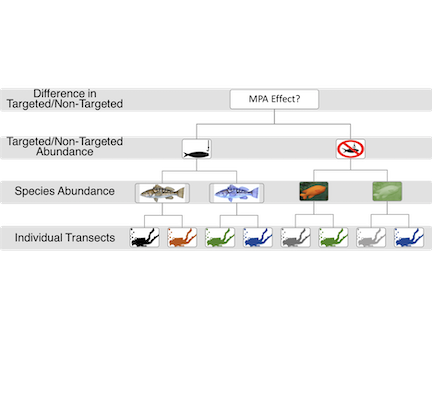
\includegraphics[width=6in]{figs/estimation-cartoon} \caption{Cartoon illustration of the hierarchichal difference-in-difference estimator}\label{fig:cartoon}
\end{figure}

\pagebreak

The first stage of the regression is a log-normal delta model. The model estimates two regressions, the first is a binomial generalized linear model (GLM) with a logit link estimating the probability of observing a given fish species at a observation \emph{i} (transect at time \emph{t}). The probability that a given species was observed \emph{o} at a given observation is distributed

\begin{equation}
o_{s,i} \sim binomial(\frac{1}{1 +e^{-\beta^{o}{X}}})
  \label{eq:binom}
\end{equation}

where \(\beta^{o}\) are the estimated coefficients for the observation model and \emph{X} is a matrix of covariates that include random effects for each year in the data (2000 to 2017).

The expected density \emph{d} of positive observations is modeled per a log-normal distribution

\begin{equation}
  log(d_{s,i}) \sim normal(\beta^{d}X, \sigma_s)
   \label{eq:logd}
 \end{equation}

where \(\beta^{d}\) are the estimated coefficients for the expected density model and \emph{X} is the same matrix of covariates as used in the observation portion of the model and \(\sigma_s\) allows for each species \emph{s} to have different standard deviations.

Our covariate matrix \emph{X} contains both fixed and random effects. Fixed effects include the depth level of the transect, the sampling site, the month of the observation, the estimated surge at the transect, visibility, the depth of the transect, and the experience (and experience squared) of the diver conducting the transect. We classify each species into one of two clusters based on the mean longitude the species was encountered at, breaking the species into two groups: those primarily found in the western end of the Channel Islands those found more in the eastern end. We then estimate random effects for each island for each cluster

\begin{equation}
\beta_{island,cluster} \sim normal(0,\sigma_{cluster})
  \label{eq:island}
\end{equation}

This allows the mean effect of each island to differ for each cluster, e.g.~allowing San Miguel, the easternmost island, to have a higher mean density for eastern species than for more western species (if the data suggest it).

The second critical component of the covariate matrix \emph{X} are random effects for each year for each species

\begin{equation}
  \beta_{year,species} \sim normal(0,\sigma_{species})
  \label{eq:species}
\end{equation}

These \(\beta_{year,species}\) represent our ``standardized'' estimate of observed abundance of each species in each time step, controlling for the included covariates.

However, we still need to account for changes in the probability of detection over time. For that, we create a standard matrix of with rows equal to the number of years and columns corresponding to each of the columns in \emph{X}, holding everything fixed at mean (or most frequently observed level for factors) levels for all variables in X except for the year and species interaction indices. Calling this standardized matrix \(X^{standard}\), the probability of observing a given species in year \emph{y} is then

\begin{equation}
p_{s,y} = (\frac{1}{1 +e^{-\beta^{o}{X^{standard}}}})
  \label{eq:pdetect}
\end{equation}

In the same manner as described by Punt et al. (2000), The standardized index of abundance for species \emph{s} in year \emph{y} then is

\begin{equation}
I_{species,year} = p_{species,year}e^{\beta_{species,year}}
  \label{eq:index}
\end{equation}

The next phase of the model requires us to estimate the mean abundance of targeted and non-targeted species over time. The concept here is that each \(I_{species,year}\) can be modeled by a regression that contains random effects for each year for targeted and non-targeted fishes, the assumption then being that there is a mean density for targeted and non-target species, and \(I_{species,year}\) represent deviations from that mean.

\begin{equation}
log(I_{species,year}) \sim normal(\beta^{effect}X^{effect}, \sigma_I)
  \label{eq:indexprior}
\end{equation}

\(X^{effect}\) contains both fixed and random effects. The fixed effects include an intercept and the temperature deviation for a given species in a year, where temperature deviation is

\begin{equation}
t_{s,y} = (t^{pref}_{s} -  \bar{t_{y}})^2
  \label{eq:tempdev}
\end{equation}

where \(t^{pref}\) is the preferred temperature for species \emph{s} (drawn form \texttt{FishLife}, Thorson et al. (2017)), and \(\bar{t_{y}}\) is the mean temperature encountered by that species in year \emph{y}. We also include as variables in the model the mean kelp cover experienced by a given species in a given year, as well as the total fishery catches reported in the previous year for that species in the Santa Barbara region {[}drawn from the California Department of Fish and Wildlife database{]}. We also include random intercepts for each species in \(X^{effect}\). The most important random effects are year effects for targeted and non-targeted species

\begin{equation}
\beta_{year,targeted} \sim normal(0,\sigma_{targeted})
  \label{eq:betatarg}
\end{equation}

\(\beta_{year,targeted}\) is the mean log density of targeted species in year \emph{y}, controlling for included covariates. Therefore, the final step in the model, the divergence in the standardized abundance trends of targeted and non-targeted species is

\begin{equation}
divergence_{year} =  \beta_{year,targeted = 1} - \beta_{year,targeted = 0}
  \label{eq:mpaeffect}
\end{equation}

The model is fit in TMB to integrate the uncertainty across all levels of the model, with standard errors for each coefficient in the model estimated through the Laplace approximation.

A complete table of estimated coefficients can be seen in Table.S\ref{tab:betatable}.

\begin{longtable}[t]{rrrl}
\caption{\label{tab:betatable}Complete table of estimated coefficients from hierarchical difference-in-difference model}\\
\toprule
estimate & lower & upper & variable\\
\midrule
\endfirsthead
\caption[]{\label{tab:betatable}Complete table of estimated coefficients from hierarchical difference-in-difference model \textit{(continued)}}\\
\toprule
estimate & lower & upper & variable\\
\midrule
\endhead
\
\endfoot
\bottomrule
\endlastfoot
0.20 & 0.15 & 0.25 & cumulative\_n\_obs\\
0.00 & -0.04 & 0.04 & surge\\
0.09 & 0.07 & 0.12 & mean\_depth\\
-0.05 & -0.08 & -0.03 & mean\_vis\\
1.47 & 1.25 & 1.69 & intercept\\
\addlinespace
-0.08 & -0.28 & 0.13 & site\_side-ANACAPA\_ADMIRALS-E\\
-0.04 & -0.23 & 0.15 & site\_side-ANACAPA\_ADMIRALS-W\\
0.10 & -0.08 & 0.27 & site\_side-ANACAPA\_BLACK\_SEA\_BASS-CEN\\
0.08 & -0.13 & 0.29 & site\_side-ANACAPA\_EAST\_FISH\_CAMP-CEN\\
-0.19 & -0.40 & 0.03 & site\_side-ANACAPA\_EAST\_FISH\_CAMP-E\\
\addlinespace
-0.34 & -0.53 & -0.14 & site\_side-ANACAPA\_EAST\_FISH\_CAMP-W\\
-0.11 & -0.26 & 0.04 & site\_side-ANACAPA\_EAST\_ISLE-CEN\\
-0.10 & -0.25 & 0.04 & site\_side-ANACAPA\_EAST\_ISLE-E\\
-0.33 & -0.47 & -0.18 & site\_side-ANACAPA\_EAST\_ISLE-W\\
0.11 & -0.05 & 0.27 & site\_side-ANACAPA\_LIGHTHOUSE\_REEF-CEN\\
\addlinespace
0.05 & -0.11 & 0.20 & site\_side-ANACAPA\_LIGHTHOUSE\_REEF-E\\
0.05 & -0.11 & 0.21 & site\_side-ANACAPA\_LIGHTHOUSE\_REEF-W\\
-0.10 & -0.25 & 0.05 & site\_side-ANACAPA\_MIDDLE\_ISLE-CEN\\
-0.27 & -0.43 & -0.12 & site\_side-ANACAPA\_MIDDLE\_ISLE-E\\
0.03 & -0.12 & 0.19 & site\_side-ANACAPA\_MIDDLE\_ISLE-W\\
\addlinespace
0.01 & -0.14 & 0.16 & site\_side-ANACAPA\_WEST\_ISLE-CEN\\
0.07 & -0.08 & 0.22 & site\_side-ANACAPA\_WEST\_ISLE-E\\
0.06 & -0.09 & 0.22 & site\_side-ANACAPA\_WEST\_ISLE-W\\
0.04 & -0.11 & 0.18 & site\_side-SCI\_CAVERN\_POINT-E\\
0.17 & 0.03 & 0.32 & site\_side-SCI\_CAVERN\_POINT-W\\
\addlinespace
0.10 & -0.05 & 0.24 & site\_side-SCI\_COCHE\_POINT-E\\
0.14 & 0.00 & 0.29 & site\_side-SCI\_COCHE\_POINT-W\\
0.09 & -0.06 & 0.24 & site\_side-SCI\_FORNEY-E\\
0.39 & 0.24 & 0.54 & site\_side-SCI\_FORNEY-W\\
0.45 & 0.30 & 0.59 & site\_side-SCI\_GULL\_ISLE-E\\
\addlinespace
0.02 & -0.13 & 0.17 & site\_side-SCI\_GULL\_ISLE-W\\
0.10 & -0.05 & 0.25 & site\_side-SCI\_HAZARDS-CEN\\
-0.23 & -0.38 & -0.08 & site\_side-SCI\_HAZARDS-E\\
0.04 & -0.11 & 0.19 & site\_side-SCI\_HAZARDS-W\\
0.25 & 0.08 & 0.42 & site\_side-SCI\_LITTLE\_SCORPION-E\\
\addlinespace
0.08 & -0.08 & 0.25 & site\_side-SCI\_LITTLE\_SCORPION-W\\
0.20 & 0.04 & 0.35 & site\_side-SCI\_PAINTED\_CAVE-CEN\\
0.30 & 0.15 & 0.45 & site\_side-SCI\_PAINTED\_CAVE-E\\
0.14 & -0.01 & 0.30 & site\_side-SCI\_PAINTED\_CAVE-W\\
0.04 & -0.10 & 0.19 & site\_side-SCI\_PELICAN-CEN\\
\addlinespace
0.28 & 0.13 & 0.43 & site\_side-SCI\_PELICAN-E\\
0.46 & 0.09 & 0.84 & site\_side-SCI\_PELICAN-FAR\_WEST\\
0.09 & -0.06 & 0.24 & site\_side-SCI\_PELICAN-W\\
0.06 & -0.11 & 0.24 & site\_side-SCI\_POTATO\_PASTURE-E\\
0.19 & 0.01 & 0.37 & site\_side-SCI\_POTATO\_PASTURE-W\\
\addlinespace
0.14 & -0.03 & 0.31 & site\_side-SCI\_SAN\_PEDRO\_POINT-E\\
0.30 & 0.14 & 0.46 & site\_side-SCI\_SAN\_PEDRO\_POINT-W\\
0.13 & -0.03 & 0.30 & site\_side-SCI\_SCORPION\_ANCHORAGE-CEN\\
0.31 & 0.16 & 0.45 & site\_side-SCI\_SCORPION-E\\
0.16 & 0.01 & 0.31 & site\_side-SCI\_SCORPION-W\\
\addlinespace
0.11 & -0.04 & 0.27 & site\_side-SCI\_VALLEY-CEN\\
0.03 & -0.15 & 0.21 & site\_side-SCI\_VALLEY-E\\
-0.09 & -0.25 & 0.07 & site\_side-SCI\_VALLEY-W\\
0.14 & -0.01 & 0.30 & site\_side-SCI\_YELLOWBANKS-CEN\\
0.14 & -0.16 & 0.44 & site\_side-SCI\_YELLOWBANKS-E\\
\addlinespace
-0.14 & -0.29 & 0.01 & site\_side-SCI\_YELLOWBANKS-W\\
0.21 & -0.19 & 0.61 & site\_side-SMI\_BAY\_POINT-CEN\\
-0.41 & -0.60 & -0.22 & site\_side-SMI\_CROOK\_POINT-E\\
0.06 & -0.12 & 0.25 & site\_side-SMI\_CROOK\_POINT-W\\
-0.15 & -0.33 & 0.04 & site\_side-SMI\_CUYLER-E\\
\addlinespace
-0.11 & -0.27 & 0.05 & site\_side-SMI\_CUYLER-W\\
0.27 & 0.11 & 0.43 & site\_side-SMI\_HARRIS\_PT\_RESERVE-E\\
0.04 & -0.13 & 0.22 & site\_side-SMI\_HARRIS\_PT\_RESERVE-W\\
0.46 & 0.29 & 0.63 & site\_side-SMI\_TYLER\_BIGHT-E\\
0.45 & 0.28 & 0.63 & site\_side-SMI\_TYLER\_BIGHT-W\\
\addlinespace
0.10 & -0.21 & 0.42 & site\_side-SRI\_BEACON\_REEF-E\\
-0.24 & -0.61 & 0.12 & site\_side-SRI\_BEACON\_REEF-W\\
-0.08 & -0.38 & 0.22 & site\_side-SRI\_BEE\_ROCK-E\\
-0.46 & -0.79 & -0.12 & site\_side-SRI\_BEE\_ROCK-W\\
-0.42 & -0.92 & 0.08 & site\_side-SRI\_CARRINGTON-CEN\\
\addlinespace
0.29 & -0.22 & 0.80 & site\_side-SRI\_CARRINGTON-E\\
0.27 & -0.12 & 0.67 & site\_side-SRI\_CARRINGTON-W\\
0.24 & 0.07 & 0.41 & site\_side-SRI\_CHICKASAW-E\\
0.26 & 0.08 & 0.43 & site\_side-SRI\_CHICKASAW-W\\
-0.10 & -0.26 & 0.06 & site\_side-SRI\_CLUSTER\_POINT-N\\
\addlinespace
-0.05 & -0.22 & 0.13 & site\_side-SRI\_CLUSTER\_POINT-S\\
0.10 & -0.26 & 0.47 & site\_side-SRI\_FORD\_POINT-CEN\\
0.02 & -0.16 & 0.20 & site\_side-SRI\_JOHNSONS\_LEE\_NORTH-E\\
-0.09 & -0.28 & 0.11 & site\_side-SRI\_JOHNSONS\_LEE\_NORTH-W\\
0.21 & 0.05 & 0.36 & site\_side-SRI\_JOHNSONS\_LEE\_SOUTH-E\\
\addlinespace
0.00 & -0.16 & 0.16 & site\_side-SRI\_JOHNSONS\_LEE\_SOUTH-W\\
-0.36 & -0.60 & -0.12 & site\_side-SRI\_JOLLA\_VIEJA-E\\
-0.28 & -0.56 & 0.00 & site\_side-SRI\_JOLLA\_VIEJA-W\\
0.24 & -0.09 & 0.58 & site\_side-SRI\_MONACOS-E\\
0.16 & -0.17 & 0.48 & site\_side-SRI\_MONACOS-W\\
\addlinespace
0.06 & -0.20 & 0.33 & site\_side-SRI\_RODES\_REEF-E\\
0.21 & -0.04 & 0.45 & site\_side-SRI\_RODES\_REEF-W\\
0.09 & -0.06 & 0.24 & site\_side-SRI\_SOUTH\_POINT-E\\
0.19 & 0.04 & 0.35 & site\_side-SRI\_SOUTH\_POINT-W\\
0.07 & -0.12 & 0.26 & site\_side-SRI\_TRANCION\_CANYON-E\\
\addlinespace
0.14 & -0.06 & 0.33 & site\_side-SRI\_TRANCION\_CANYON-W\\
-0.03 & -0.09 & 0.02 & level-CNMD\\
0.03 & -0.01 & 0.06 & level-MID\\
0.00 & -0.05 & 0.05 & factor\_month-11\\
0.14 & 0.07 & 0.21 & factor\_month-12\\
\addlinespace
-0.28 & -0.50 & -0.07 & factor\_month-7\\
-0.02 & -0.06 & 0.02 & factor\_month-8\\
-0.02 & -0.05 & 0.01 & factor\_month-9\\
-0.05 & -0.11 & 0.01 & cumulative\_n\_obs\_2\\
0.42 & 0.36 & 0.48 & cumulative\_n\_obs\\
\addlinespace
-0.04 & -0.09 & 0.00 & surge\\
-0.26 & -0.29 & -0.23 & mean\_depth\\
0.09 & 0.06 & 0.11 & mean\_vis\\
-0.59 & -0.76 & -0.42 & intercept\\
-0.38 & -0.60 & -0.16 & site\_side-ANACAPA\_ADMIRALS-E\\
\addlinespace
-0.16 & -0.37 & 0.06 & site\_side-ANACAPA\_ADMIRALS-W\\
-0.39 & -0.58 & -0.19 & site\_side-ANACAPA\_BLACK\_SEA\_BASS-CEN\\
-0.46 & -0.70 & -0.23 & site\_side-ANACAPA\_EAST\_FISH\_CAMP-CEN\\
-0.52 & -0.75 & -0.28 & site\_side-ANACAPA\_EAST\_FISH\_CAMP-E\\
-0.27 & -0.49 & -0.05 & site\_side-ANACAPA\_EAST\_FISH\_CAMP-W\\
\addlinespace
0.27 & 0.10 & 0.44 & site\_side-ANACAPA\_EAST\_ISLE-CEN\\
0.34 & 0.18 & 0.51 & site\_side-ANACAPA\_EAST\_ISLE-E\\
-0.05 & -0.22 & 0.12 & site\_side-ANACAPA\_EAST\_ISLE-W\\
-0.27 & -0.45 & -0.09 & site\_side-ANACAPA\_LIGHTHOUSE\_REEF-CEN\\
-0.03 & -0.21 & 0.15 & site\_side-ANACAPA\_LIGHTHOUSE\_REEF-E\\
\addlinespace
-0.21 & -0.39 & -0.03 & site\_side-ANACAPA\_LIGHTHOUSE\_REEF-W\\
-0.18 & -0.35 & -0.01 & site\_side-ANACAPA\_MIDDLE\_ISLE-CEN\\
-0.48 & -0.65 & -0.31 & site\_side-ANACAPA\_MIDDLE\_ISLE-E\\
-0.49 & -0.67 & -0.32 & site\_side-ANACAPA\_MIDDLE\_ISLE-W\\
0.07 & -0.10 & 0.24 & site\_side-ANACAPA\_WEST\_ISLE-CEN\\
\addlinespace
-0.06 & -0.23 & 0.11 & site\_side-ANACAPA\_WEST\_ISLE-E\\
-0.34 & -0.51 & -0.16 & site\_side-ANACAPA\_WEST\_ISLE-W\\
0.11 & -0.06 & 0.27 & site\_side-SCI\_CAVERN\_POINT-E\\
0.12 & -0.04 & 0.29 & site\_side-SCI\_CAVERN\_POINT-W\\
0.20 & 0.03 & 0.36 & site\_side-SCI\_COCHE\_POINT-E\\
\addlinespace
-0.01 & -0.17 & 0.16 & site\_side-SCI\_COCHE\_POINT-W\\
-0.50 & -0.67 & -0.34 & site\_side-SCI\_FORNEY-E\\
-0.36 & -0.52 & -0.19 & site\_side-SCI\_FORNEY-W\\
0.19 & 0.03 & 0.35 & site\_side-SCI\_GULL\_ISLE-E\\
-0.08 & -0.24 & 0.09 & site\_side-SCI\_GULL\_ISLE-W\\
\addlinespace
0.06 & -0.11 & 0.23 & site\_side-SCI\_HAZARDS-CEN\\
0.03 & -0.14 & 0.19 & site\_side-SCI\_HAZARDS-E\\
0.07 & -0.10 & 0.23 & site\_side-SCI\_HAZARDS-W\\
-0.02 & -0.21 & 0.18 & site\_side-SCI\_LITTLE\_SCORPION-E\\
0.28 & 0.09 & 0.47 & site\_side-SCI\_LITTLE\_SCORPION-W\\
\addlinespace
0.05 & -0.12 & 0.22 & site\_side-SCI\_PAINTED\_CAVE-CEN\\
0.16 & -0.01 & 0.33 & site\_side-SCI\_PAINTED\_CAVE-E\\
-0.13 & -0.30 & 0.05 & site\_side-SCI\_PAINTED\_CAVE-W\\
0.15 & -0.01 & 0.32 & site\_side-SCI\_PELICAN-CEN\\
0.17 & 0.00 & 0.34 & site\_side-SCI\_PELICAN-E\\
\addlinespace
-0.07 & -0.47 & 0.32 & site\_side-SCI\_PELICAN-FAR\_WEST\\
-0.12 & -0.29 & 0.04 & site\_side-SCI\_PELICAN-W\\
-0.29 & -0.49 & -0.09 & site\_side-SCI\_POTATO\_PASTURE-E\\
-0.34 & -0.54 & -0.15 & site\_side-SCI\_POTATO\_PASTURE-W\\
-0.24 & -0.44 & -0.05 & site\_side-SCI\_SAN\_PEDRO\_POINT-E\\
\addlinespace
0.25 & 0.06 & 0.43 & site\_side-SCI\_SAN\_PEDRO\_POINT-W\\
-0.06 & -0.25 & 0.13 & site\_side-SCI\_SCORPION\_ANCHORAGE-CEN\\
0.05 & -0.12 & 0.21 & site\_side-SCI\_SCORPION-E\\
-0.16 & -0.33 & 0.00 & site\_side-SCI\_SCORPION-W\\
-0.21 & -0.39 & -0.04 & site\_side-SCI\_VALLEY-CEN\\
\addlinespace
-0.95 & -1.14 & -0.76 & site\_side-SCI\_VALLEY-E\\
-0.58 & -0.76 & -0.40 & site\_side-SCI\_VALLEY-W\\
-0.58 & -0.75 & -0.41 & site\_side-SCI\_YELLOWBANKS-CEN\\
-0.65 & -0.97 & -0.34 & site\_side-SCI\_YELLOWBANKS-E\\
-0.43 & -0.59 & -0.26 & site\_side-SCI\_YELLOWBANKS-W\\
\addlinespace
-0.56 & -0.97 & -0.14 & site\_side-SMI\_BAY\_POINT-CEN\\
-1.52 & -1.71 & -1.32 & site\_side-SMI\_CROOK\_POINT-E\\
-1.36 & -1.55 & -1.17 & site\_side-SMI\_CROOK\_POINT-W\\
-1.67 & -1.86 & -1.48 & site\_side-SMI\_CUYLER-E\\
-0.97 & -1.14 & -0.79 & site\_side-SMI\_CUYLER-W\\
\addlinespace
-0.57 & -0.75 & -0.40 & site\_side-SMI\_HARRIS\_PT\_RESERVE-E\\
-1.43 & -1.62 & -1.25 & site\_side-SMI\_HARRIS\_PT\_RESERVE-W\\
-0.68 & -0.86 & -0.50 & site\_side-SMI\_TYLER\_BIGHT-E\\
-1.00 & -1.18 & -0.82 & site\_side-SMI\_TYLER\_BIGHT-W\\
-1.58 & -1.88 & -1.28 & site\_side-SRI\_BEACON\_REEF-E\\
\addlinespace
-1.77 & -2.12 & -1.43 & site\_side-SRI\_BEACON\_REEF-W\\
-1.08 & -1.37 & -0.80 & site\_side-SRI\_BEE\_ROCK-E\\
-1.16 & -1.46 & -0.85 & site\_side-SRI\_BEE\_ROCK-W\\
-1.21 & -1.67 & -0.74 & site\_side-SRI\_CARRINGTON-CEN\\
-1.29 & -1.76 & -0.82 & site\_side-SRI\_CARRINGTON-E\\
\addlinespace
-1.26 & -1.63 & -0.88 & site\_side-SRI\_CARRINGTON-W\\
-0.40 & -0.58 & -0.21 & site\_side-SRI\_CHICKASAW-E\\
-0.62 & -0.80 & -0.43 & site\_side-SRI\_CHICKASAW-W\\
-0.88 & -1.05 & -0.70 & site\_side-SRI\_CLUSTER\_POINT-N\\
-1.31 & -1.49 & -1.12 & site\_side-SRI\_CLUSTER\_POINT-S\\
\addlinespace
-0.74 & -1.09 & -0.39 & site\_side-SRI\_FORD\_POINT-CEN\\
-0.64 & -0.83 & -0.45 & site\_side-SRI\_JOHNSONS\_LEE\_NORTH-E\\
-0.92 & -1.11 & -0.72 & site\_side-SRI\_JOHNSONS\_LEE\_NORTH-W\\
-0.35 & -0.51 & -0.18 & site\_side-SRI\_JOHNSONS\_LEE\_SOUTH-E\\
-0.96 & -1.13 & -0.79 & site\_side-SRI\_JOHNSONS\_LEE\_SOUTH-W\\
\addlinespace
-0.82 & -1.06 & -0.58 & site\_side-SRI\_JOLLA\_VIEJA-E\\
-1.31 & -1.57 & -1.04 & site\_side-SRI\_JOLLA\_VIEJA-W\\
-1.25 & -1.55 & -0.95 & site\_side-SRI\_MONACOS-E\\
-0.76 & -1.06 & -0.46 & site\_side-SRI\_MONACOS-W\\
-0.83 & -1.09 & -0.56 & site\_side-SRI\_RODES\_REEF-E\\
\addlinespace
-0.92 & -1.17 & -0.68 & site\_side-SRI\_RODES\_REEF-W\\
-0.66 & -0.83 & -0.49 & site\_side-SRI\_SOUTH\_POINT-E\\
-0.58 & -0.75 & -0.41 & site\_side-SRI\_SOUTH\_POINT-W\\
-0.87 & -1.07 & -0.68 & site\_side-SRI\_TRANCION\_CANYON-E\\
-0.88 & -1.08 & -0.69 & site\_side-SRI\_TRANCION\_CANYON-W\\
\addlinespace
-1.63 & -1.68 & -1.57 & level-CNMD\\
-1.46 & -1.50 & -1.43 & level-MID\\
0.01 & -0.04 & 0.06 & factor\_month-11\\
-0.10 & -0.17 & -0.03 & factor\_month-12\\
-0.01 & -0.24 & 0.23 & factor\_month-7\\
\addlinespace
0.09 & 0.05 & 0.13 & factor\_month-8\\
0.12 & 0.09 & 0.16 & factor\_month-9\\
-0.22 & -0.27 & -0.16 & cumulative\_n\_obs\_2\\
-1.18 & -1.71 & -0.65 & year\_classcode-bfre-2000\\
-0.62 & -1.11 & -0.12 & year\_classcode-bfre-2001\\
\addlinespace
-1.48 & -1.95 & -1.01 & year\_classcode-bfre-2002\\
-2.25 & -2.56 & -1.95 & year\_classcode-bfre-2003\\
-1.86 & -2.11 & -1.62 & year\_classcode-bfre-2004\\
-2.03 & -2.26 & -1.80 & year\_classcode-bfre-2005\\
-2.26 & -2.51 & -2.02 & year\_classcode-bfre-2006\\
\addlinespace
-1.81 & -2.04 & -1.58 & year\_classcode-bfre-2007\\
-2.53 & -2.81 & -2.25 & year\_classcode-bfre-2008\\
-2.17 & -2.39 & -1.95 & year\_classcode-bfre-2009\\
-2.42 & -2.68 & -2.17 & year\_classcode-bfre-2010\\
-2.18 & -2.45 & -1.91 & year\_classcode-bfre-2011\\
\addlinespace
-2.30 & -2.56 & -2.03 & year\_classcode-bfre-2012\\
-2.17 & -2.43 & -1.92 & year\_classcode-bfre-2013\\
-1.87 & -2.13 & -1.61 & year\_classcode-bfre-2014\\
-2.52 & -2.81 & -2.23 & year\_classcode-bfre-2015\\
-2.67 & -3.07 & -2.26 & year\_classcode-bfre-2016\\
\addlinespace
-2.39 & -2.71 & -2.08 & year\_classcode-bfre-2017\\
1.07 & 0.48 & 1.66 & year\_classcode-cpri-2000\\
0.67 & 0.00 & 1.33 & year\_classcode-cpri-2001\\
0.64 & -0.02 & 1.29 & year\_classcode-cpri-2002\\
0.60 & 0.10 & 1.10 & year\_classcode-cpri-2003\\
\addlinespace
0.67 & 0.15 & 1.19 & year\_classcode-cpri-2004\\
0.57 & 0.14 & 0.99 & year\_classcode-cpri-2005\\
0.59 & 0.11 & 1.07 & year\_classcode-cpri-2006\\
0.83 & 0.35 & 1.32 & year\_classcode-cpri-2007\\
0.77 & 0.30 & 1.24 & year\_classcode-cpri-2008\\
\addlinespace
1.06 & 0.64 & 1.48 & year\_classcode-cpri-2009\\
1.01 & 0.55 & 1.48 & year\_classcode-cpri-2010\\
1.33 & 0.80 & 1.85 & year\_classcode-cpri-2011\\
1.48 & 0.94 & 2.02 & year\_classcode-cpri-2012\\
1.07 & 0.43 & 1.72 & year\_classcode-cpri-2013\\
\addlinespace
1.10 & 0.53 & 1.68 & year\_classcode-cpri-2014\\
-1.32 & -1.73 & -0.91 & year\_classcode-cpri-2015\\
0.12 & -0.20 & 0.44 & year\_classcode-cpri-2016\\
0.46 & 0.13 & 0.79 & year\_classcode-cpri-2017\\
1.23 & 0.88 & 1.58 & year\_classcode-cpun-2000\\
\addlinespace
1.02 & 0.68 & 1.37 & year\_classcode-cpun-2001\\
0.39 & 0.10 & 0.68 & year\_classcode-cpun-2002\\
0.14 & -0.10 & 0.38 & year\_classcode-cpun-2003\\
-0.30 & -0.54 & -0.07 & year\_classcode-cpun-2004\\
-0.25 & -0.46 & -0.04 & year\_classcode-cpun-2005\\
\addlinespace
-0.41 & -0.63 & -0.20 & year\_classcode-cpun-2006\\
-0.37 & -0.58 & -0.15 & year\_classcode-cpun-2007\\
-0.73 & -0.95 & -0.52 & year\_classcode-cpun-2008\\
0.16 & -0.05 & 0.36 & year\_classcode-cpun-2009\\
0.17 & -0.05 & 0.39 & year\_classcode-cpun-2010\\
\addlinespace
0.35 & 0.12 & 0.58 & year\_classcode-cpun-2011\\
0.16 & -0.07 & 0.39 & year\_classcode-cpun-2012\\
0.13 & -0.11 & 0.36 & year\_classcode-cpun-2013\\
-0.24 & -0.47 & -0.02 & year\_classcode-cpun-2014\\
-0.36 & -0.57 & -0.14 & year\_classcode-cpun-2015\\
\addlinespace
0.04 & -0.17 & 0.25 & year\_classcode-cpun-2016\\
-0.22 & -0.44 & 0.00 & year\_classcode-cpun-2017\\
0.66 & 0.27 & 1.05 & year\_classcode-ejac-2000\\
0.41 & 0.01 & 0.81 & year\_classcode-ejac-2001\\
0.48 & 0.13 & 0.82 & year\_classcode-ejac-2002\\
\addlinespace
-0.18 & -0.45 & 0.10 & year\_classcode-ejac-2003\\
-0.42 & -0.68 & -0.17 & year\_classcode-ejac-2004\\
-0.07 & -0.29 & 0.16 & year\_classcode-ejac-2005\\
0.31 & 0.08 & 0.54 & year\_classcode-ejac-2006\\
-0.09 & -0.32 & 0.13 & year\_classcode-ejac-2007\\
\addlinespace
-0.90 & -1.13 & -0.67 & year\_classcode-ejac-2008\\
-0.13 & -0.35 & 0.09 & year\_classcode-ejac-2009\\
-0.05 & -0.28 & 0.18 & year\_classcode-ejac-2010\\
-0.01 & -0.25 & 0.22 & year\_classcode-ejac-2011\\
-0.44 & -0.68 & -0.20 & year\_classcode-ejac-2012\\
\addlinespace
-0.28 & -0.54 & -0.03 & year\_classcode-ejac-2013\\
-0.23 & -0.48 & 0.01 & year\_classcode-ejac-2014\\
-0.53 & -0.79 & -0.28 & year\_classcode-ejac-2015\\
-0.50 & -0.76 & -0.24 & year\_classcode-ejac-2016\\
-0.84 & -1.09 & -0.58 & year\_classcode-ejac-2017\\
\addlinespace
0.11 & -0.47 & 0.68 & year\_classcode-elat-2000\\
0.29 & -0.27 & 0.85 & year\_classcode-elat-2001\\
0.23 & -0.28 & 0.74 & year\_classcode-elat-2002\\
0.28 & -0.03 & 0.59 & year\_classcode-elat-2003\\
-0.26 & -0.52 & 0.01 & year\_classcode-elat-2004\\
\addlinespace
-0.26 & -0.48 & -0.04 & year\_classcode-elat-2005\\
0.27 & 0.05 & 0.49 & year\_classcode-elat-2006\\
0.12 & -0.12 & 0.37 & year\_classcode-elat-2007\\
-0.73 & -0.96 & -0.49 & year\_classcode-elat-2008\\
0.12 & -0.09 & 0.33 & year\_classcode-elat-2009\\
\addlinespace
0.05 & -0.18 & 0.28 & year\_classcode-elat-2010\\
0.02 & -0.20 & 0.25 & year\_classcode-elat-2011\\
-0.06 & -0.29 & 0.16 & year\_classcode-elat-2012\\
-0.18 & -0.46 & 0.10 & year\_classcode-elat-2013\\
-0.20 & -0.44 & 0.03 & year\_classcode-elat-2014\\
\addlinespace
-0.07 & -0.38 & 0.24 & year\_classcode-elat-2015\\
-0.70 & -1.04 & -0.37 & year\_classcode-elat-2016\\
-0.82 & -1.18 & -0.47 & year\_classcode-elat-2017\\
1.46 & 1.06 & 1.85 & year\_classcode-gnig-2000\\
1.48 & 1.11 & 1.86 & year\_classcode-gnig-2001\\
\addlinespace
1.25 & 0.92 & 1.59 & year\_classcode-gnig-2002\\
1.33 & 1.06 & 1.60 & year\_classcode-gnig-2003\\
1.01 & 0.77 & 1.25 & year\_classcode-gnig-2004\\
1.20 & 0.98 & 1.42 & year\_classcode-gnig-2005\\
1.22 & 1.00 & 1.44 & year\_classcode-gnig-2006\\
\addlinespace
1.27 & 1.05 & 1.49 & year\_classcode-gnig-2007\\
1.02 & 0.80 & 1.24 & year\_classcode-gnig-2008\\
1.32 & 1.10 & 1.53 & year\_classcode-gnig-2009\\
1.46 & 1.21 & 1.70 & year\_classcode-gnig-2010\\
1.34 & 1.10 & 1.59 & year\_classcode-gnig-2011\\
\addlinespace
1.46 & 1.22 & 1.71 & year\_classcode-gnig-2012\\
1.21 & 0.94 & 1.48 & year\_classcode-gnig-2013\\
1.28 & 1.04 & 1.52 & year\_classcode-gnig-2014\\
1.11 & 0.88 & 1.34 & year\_classcode-gnig-2015\\
1.31 & 1.07 & 1.55 & year\_classcode-gnig-2016\\
\addlinespace
1.29 & 1.06 & 1.52 & year\_classcode-gnig-2017\\
-0.39 & -1.89 & 1.10 & year\_classcode-hcar-2000\\
-1.50 & -2.40 & -0.61 & year\_classcode-hcar-2001\\
-1.99 & -2.70 & -1.28 & year\_classcode-hcar-2002\\
-1.44 & -1.93 & -0.95 & year\_classcode-hcar-2003\\
\addlinespace
-1.38 & -1.98 & -0.78 & year\_classcode-hcar-2004\\
-1.47 & -1.80 & -1.15 & year\_classcode-hcar-2005\\
-1.98 & -2.31 & -1.65 & year\_classcode-hcar-2006\\
-1.59 & -1.88 & -1.29 & year\_classcode-hcar-2007\\
-2.68 & -2.98 & -2.37 & year\_classcode-hcar-2008\\
\addlinespace
-1.61 & -1.92 & -1.31 & year\_classcode-hcar-2009\\
-1.73 & -2.11 & -1.36 & year\_classcode-hcar-2010\\
-1.56 & -2.11 & -1.01 & year\_classcode-hcar-2011\\
-1.90 & -2.34 & -1.46 & year\_classcode-hcar-2012\\
-2.00 & -2.47 & -1.53 & year\_classcode-hcar-2013\\
\addlinespace
-1.87 & -2.58 & -1.17 & year\_classcode-hcar-2014\\
-0.87 & -1.79 & 0.05 & year\_classcode-hcar-2015\\
-1.37 & -2.23 & -0.51 & year\_classcode-hcar-2016\\
-1.40 & -2.19 & -0.62 & year\_classcode-hcar-2017\\
-2.80 & -3.71 & -1.89 & year\_classcode-hros-2000\\
\addlinespace
-3.55 & -4.28 & -2.82 & year\_classcode-hros-2001\\
-2.91 & -3.86 & -1.97 & year\_classcode-hros-2002\\
-2.59 & -3.53 & -1.65 & year\_classcode-hros-2003\\
-4.13 & -4.46 & -3.80 & year\_classcode-hros-2004\\
-3.71 & -4.10 & -3.32 & year\_classcode-hros-2005\\
\addlinespace
-4.09 & -4.49 & -3.69 & year\_classcode-hros-2006\\
-3.89 & -4.23 & -3.56 & year\_classcode-hros-2007\\
-4.28 & -4.76 & -3.79 & year\_classcode-hros-2008\\
-3.66 & -3.97 & -3.36 & year\_classcode-hros-2009\\
-1.29 & -2.20 & -0.39 & year\_classcode-hros-2010\\
\addlinespace
-3.54 & -4.02 & -3.06 & year\_classcode-hros-2011\\
-3.59 & -3.99 & -3.18 & year\_classcode-hros-2012\\
-2.25 & -3.11 & -1.39 & year\_classcode-hros-2013\\
-3.54 & -4.02 & -3.06 & year\_classcode-hros-2014\\
-3.31 & -3.81 & -2.81 & year\_classcode-hros-2015\\
\addlinespace
-2.57 & -3.11 & -2.04 & year\_classcode-hros-2016\\
-3.94 & -4.32 & -3.57 & year\_classcode-hros-2017\\
1.73 & 1.38 & 2.07 & year\_classcode-hrub-2000\\
1.78 & 1.47 & 2.10 & year\_classcode-hrub-2001\\
1.47 & 1.18 & 1.77 & year\_classcode-hrub-2002\\
\addlinespace
1.37 & 1.10 & 1.63 & year\_classcode-hrub-2003\\
0.89 & 0.66 & 1.13 & year\_classcode-hrub-2004\\
1.03 & 0.82 & 1.25 & year\_classcode-hrub-2005\\
0.95 & 0.73 & 1.16 & year\_classcode-hrub-2006\\
1.10 & 0.88 & 1.31 & year\_classcode-hrub-2007\\
\addlinespace
0.89 & 0.67 & 1.10 & year\_classcode-hrub-2008\\
1.18 & 0.97 & 1.39 & year\_classcode-hrub-2009\\
1.07 & 0.83 & 1.31 & year\_classcode-hrub-2010\\
1.00 & 0.76 & 1.23 & year\_classcode-hrub-2011\\
1.05 & 0.82 & 1.29 & year\_classcode-hrub-2012\\
\addlinespace
1.02 & 0.78 & 1.26 & year\_classcode-hrub-2013\\
0.34 & 0.12 & 0.57 & year\_classcode-hrub-2014\\
0.49 & 0.27 & 0.71 & year\_classcode-hrub-2015\\
0.36 & 0.14 & 0.58 & year\_classcode-hrub-2016\\
0.70 & 0.48 & 0.91 & year\_classcode-hrub-2017\\
\addlinespace
-0.10 & -0.45 & 0.25 & year\_classcode-hsem-2000\\
0.04 & -0.34 & 0.41 & year\_classcode-hsem-2001\\
-0.29 & -0.68 & 0.11 & year\_classcode-hsem-2002\\
-0.49 & -0.90 & -0.08 & year\_classcode-hsem-2003\\
-0.31 & -0.68 & 0.06 & year\_classcode-hsem-2004\\
\addlinespace
-1.33 & -1.59 & -1.07 & year\_classcode-hsem-2005\\
-0.85 & -1.13 & -0.57 & year\_classcode-hsem-2006\\
-1.16 & -1.39 & -0.93 & year\_classcode-hsem-2007\\
-1.03 & -1.27 & -0.80 & year\_classcode-hsem-2008\\
-0.56 & -0.78 & -0.33 & year\_classcode-hsem-2009\\
\addlinespace
-0.40 & -0.68 & -0.12 & year\_classcode-hsem-2010\\
-0.26 & -0.55 & 0.02 & year\_classcode-hsem-2011\\
-0.13 & -0.52 & 0.27 & year\_classcode-hsem-2012\\
-0.75 & -1.16 & -0.34 & year\_classcode-hsem-2013\\
-1.88 & -2.17 & -1.59 & year\_classcode-hsem-2014\\
\addlinespace
-0.56 & -0.77 & -0.34 & year\_classcode-hsem-2015\\
-0.19 & -0.40 & 0.02 & year\_classcode-hsem-2016\\
-0.13 & -0.35 & 0.08 & year\_classcode-hsem-2017\\
0.87 & 0.43 & 1.32 & year\_classcode-mcal-2000\\
0.99 & 0.58 & 1.39 & year\_classcode-mcal-2001\\
\addlinespace
0.27 & -0.07 & 0.62 & year\_classcode-mcal-2002\\
0.47 & 0.18 & 0.77 & year\_classcode-mcal-2003\\
-0.05 & -0.32 & 0.22 & year\_classcode-mcal-2004\\
0.12 & -0.11 & 0.34 & year\_classcode-mcal-2005\\
-0.15 & -0.36 & 0.06 & year\_classcode-mcal-2006\\
\addlinespace
0.30 & 0.07 & 0.53 & year\_classcode-mcal-2007\\
-0.15 & -0.39 & 0.09 & year\_classcode-mcal-2008\\
0.43 & 0.19 & 0.68 & year\_classcode-mcal-2009\\
0.67 & 0.36 & 0.98 & year\_classcode-mcal-2010\\
0.44 & 0.11 & 0.76 & year\_classcode-mcal-2011\\
\addlinespace
0.71 & 0.36 & 1.07 & year\_classcode-mcal-2012\\
0.49 & 0.13 & 0.84 & year\_classcode-mcal-2013\\
0.11 & -0.14 & 0.36 & year\_classcode-mcal-2014\\
-0.07 & -0.29 & 0.14 & year\_classcode-mcal-2015\\
0.32 & 0.10 & 0.54 & year\_classcode-mcal-2016\\
\addlinespace
0.05 & -0.17 & 0.28 & year\_classcode-mcal-2017\\
0.23 & -0.13 & 0.59 & year\_classcode-ocal-2000\\
0.16 & -0.19 & 0.51 & year\_classcode-ocal-2001\\
-0.36 & -0.69 & -0.03 & year\_classcode-ocal-2002\\
-0.96 & -1.20 & -0.71 & year\_classcode-ocal-2003\\
\addlinespace
-0.93 & -1.15 & -0.70 & year\_classcode-ocal-2004\\
-0.81 & -1.02 & -0.61 & year\_classcode-ocal-2005\\
-0.45 & -0.66 & -0.25 & year\_classcode-ocal-2006\\
-0.50 & -0.71 & -0.30 & year\_classcode-ocal-2007\\
-0.94 & -1.14 & -0.73 & year\_classcode-ocal-2008\\
\addlinespace
-0.19 & -0.38 & 0.01 & year\_classcode-ocal-2009\\
-0.19 & -0.40 & 0.01 & year\_classcode-ocal-2010\\
-0.42 & -0.64 & -0.20 & year\_classcode-ocal-2011\\
-0.62 & -0.83 & -0.40 & year\_classcode-ocal-2012\\
-0.46 & -0.69 & -0.22 & year\_classcode-ocal-2013\\
\addlinespace
-0.65 & -0.87 & -0.44 & year\_classcode-ocal-2014\\
-0.71 & -0.92 & -0.50 & year\_classcode-ocal-2015\\
-0.63 & -0.84 & -0.41 & year\_classcode-ocal-2016\\
-0.57 & -0.79 & -0.35 & year\_classcode-ocal-2017\\
-1.12 & -1.60 & -0.64 & year\_classcode-opic-2000\\
\addlinespace
-1.72 & -2.17 & -1.28 & year\_classcode-opic-2001\\
0.23 & -0.84 & 1.30 & year\_classcode-opic-2002\\
-1.93 & -2.30 & -1.56 & year\_classcode-opic-2003\\
-1.68 & -1.91 & -1.46 & year\_classcode-opic-2004\\
-1.91 & -2.12 & -1.70 & year\_classcode-opic-2005\\
\addlinespace
-1.70 & -1.92 & -1.48 & year\_classcode-opic-2006\\
-2.09 & -2.30 & -1.88 & year\_classcode-opic-2007\\
-2.19 & -2.40 & -1.99 & year\_classcode-opic-2008\\
-2.07 & -2.27 & -1.87 & year\_classcode-opic-2009\\
-1.94 & -2.15 & -1.74 & year\_classcode-opic-2010\\
\addlinespace
-1.84 & -2.05 & -1.64 & year\_classcode-opic-2011\\
-1.80 & -2.01 & -1.60 & year\_classcode-opic-2012\\
-2.06 & -2.28 & -1.85 & year\_classcode-opic-2013\\
-2.35 & -2.56 & -2.13 & year\_classcode-opic-2014\\
-2.49 & -2.75 & -2.23 & year\_classcode-opic-2015\\
\addlinespace
-2.52 & -2.76 & -2.27 & year\_classcode-opic-2016\\
-2.39 & -2.64 & -2.14 & year\_classcode-opic-2017\\
1.39 & 1.07 & 1.71 & year\_classcode-pcla-2000\\
1.45 & 1.14 & 1.75 & year\_classcode-pcla-2001\\
1.26 & 0.98 & 1.53 & year\_classcode-pcla-2002\\
\addlinespace
0.86 & 0.61 & 1.11 & year\_classcode-pcla-2003\\
0.56 & 0.34 & 0.79 & year\_classcode-pcla-2004\\
0.03 & -0.17 & 0.24 & year\_classcode-pcla-2005\\
0.26 & 0.05 & 0.47 & year\_classcode-pcla-2006\\
0.46 & 0.26 & 0.67 & year\_classcode-pcla-2007\\
\addlinespace
0.35 & 0.14 & 0.55 & year\_classcode-pcla-2008\\
0.98 & 0.78 & 1.18 & year\_classcode-pcla-2009\\
0.83 & 0.61 & 1.06 & year\_classcode-pcla-2010\\
1.01 & 0.79 & 1.23 & year\_classcode-pcla-2011\\
1.02 & 0.80 & 1.24 & year\_classcode-pcla-2012\\
\addlinespace
0.86 & 0.63 & 1.08 & year\_classcode-pcla-2013\\
0.54 & 0.33 & 0.76 & year\_classcode-pcla-2014\\
0.49 & 0.28 & 0.70 & year\_classcode-pcla-2015\\
0.65 & 0.44 & 0.86 & year\_classcode-pcla-2016\\
0.78 & 0.58 & 0.99 & year\_classcode-pcla-2017\\
\addlinespace
-0.76 & -2.00 & 0.48 & year\_classcode-pfur-2000\\
-0.92 & -2.05 & 0.22 & year\_classcode-pfur-2001\\
-0.54 & -1.89 & 0.82 & year\_classcode-pfur-2002\\
-1.25 & -2.15 & -0.35 & year\_classcode-pfur-2003\\
-1.84 & -2.61 & -1.06 & year\_classcode-pfur-2004\\
\addlinespace
-0.67 & -1.37 & 0.03 & year\_classcode-pfur-2005\\
-1.00 & -1.74 & -0.26 & year\_classcode-pfur-2006\\
-0.67 & -1.74 & 0.39 & year\_classcode-pfur-2007\\
-1.52 & -2.54 & -0.51 & year\_classcode-pfur-2008\\
-1.45 & -2.10 & -0.79 & year\_classcode-pfur-2009\\
\addlinespace
-0.92 & -1.70 & -0.15 & year\_classcode-pfur-2010\\
-0.47 & -1.42 & 0.48 & year\_classcode-pfur-2011\\
-0.64 & -1.79 & 0.51 & year\_classcode-pfur-2012\\
0.37 & -1.00 & 1.75 & year\_classcode-pfur-2013\\
-0.75 & -1.83 & 0.33 & year\_classcode-pfur-2014\\
\addlinespace
0.51 & -0.83 & 1.86 & year\_classcode-pfur-2015\\
0.13 & -1.13 & 1.39 & year\_classcode-pfur-2016\\
-0.11 & -1.36 & 1.14 & year\_classcode-pfur-2017\\
0.95 & 0.13 & 1.77 & year\_classcode-rtox-2000\\
1.10 & 0.51 & 1.69 & year\_classcode-rtox-2001\\
\addlinespace
0.81 & 0.34 & 1.29 & year\_classcode-rtox-2002\\
0.79 & 0.36 & 1.22 & year\_classcode-rtox-2003\\
0.68 & 0.27 & 1.08 & year\_classcode-rtox-2004\\
0.94 & 0.61 & 1.26 & year\_classcode-rtox-2005\\
0.87 & 0.52 & 1.23 & year\_classcode-rtox-2006\\
\addlinespace
1.26 & 0.90 & 1.62 & year\_classcode-rtox-2007\\
1.40 & 0.96 & 1.83 & year\_classcode-rtox-2008\\
1.31 & 1.01 & 1.61 & year\_classcode-rtox-2009\\
1.12 & 0.78 & 1.47 & year\_classcode-rtox-2010\\
0.79 & 0.48 & 1.11 & year\_classcode-rtox-2011\\
\addlinespace
0.93 & 0.56 & 1.29 & year\_classcode-rtox-2012\\
0.90 & 0.49 & 1.31 & year\_classcode-rtox-2013\\
1.47 & 1.01 & 1.92 & year\_classcode-rtox-2014\\
0.51 & 0.07 & 0.95 & year\_classcode-rtox-2015\\
0.54 & 0.11 & 0.98 & year\_classcode-rtox-2016\\
\addlinespace
-0.18 & -0.78 & 0.41 & year\_classcode-rtox-2017\\
0.27 & -0.15 & 0.68 & year\_classcode-rvac-2000\\
0.29 & -0.11 & 0.70 & year\_classcode-rvac-2001\\
0.05 & -0.31 & 0.41 & year\_classcode-rvac-2002\\
-0.27 & -0.57 & 0.02 & year\_classcode-rvac-2003\\
\addlinespace
-0.39 & -0.68 & -0.10 & year\_classcode-rvac-2004\\
-0.12 & -0.36 & 0.12 & year\_classcode-rvac-2005\\
0.28 & 0.04 & 0.51 & year\_classcode-rvac-2006\\
-0.08 & -0.32 & 0.17 & year\_classcode-rvac-2007\\
-0.49 & -0.77 & -0.22 & year\_classcode-rvac-2008\\
\addlinespace
-0.20 & -0.44 & 0.04 & year\_classcode-rvac-2009\\
-0.13 & -0.38 & 0.11 & year\_classcode-rvac-2010\\
0.00 & -0.25 & 0.25 & year\_classcode-rvac-2011\\
-0.45 & -0.72 & -0.18 & year\_classcode-rvac-2012\\
0.16 & -0.13 & 0.45 & year\_classcode-rvac-2013\\
\addlinespace
-0.13 & -0.41 & 0.15 & year\_classcode-rvac-2014\\
-0.36 & -0.68 & -0.05 & year\_classcode-rvac-2015\\
-0.14 & -0.44 & 0.17 & year\_classcode-rvac-2016\\
-0.67 & -1.00 & -0.34 & year\_classcode-rvac-2017\\
0.78 & 0.24 & 1.31 & year\_classcode-satr-2000\\
\addlinespace
0.87 & 0.41 & 1.32 & year\_classcode-satr-2001\\
0.69 & 0.29 & 1.10 & year\_classcode-satr-2002\\
0.35 & 0.08 & 0.61 & year\_classcode-satr-2003\\
0.02 & -0.21 & 0.26 & year\_classcode-satr-2004\\
0.00 & -0.21 & 0.20 & year\_classcode-satr-2005\\
\addlinespace
0.39 & 0.18 & 0.59 & year\_classcode-satr-2006\\
0.25 & 0.04 & 0.45 & year\_classcode-satr-2007\\
-0.10 & -0.31 & 0.10 & year\_classcode-satr-2008\\
0.50 & 0.31 & 0.69 & year\_classcode-satr-2009\\
0.30 & 0.09 & 0.51 & year\_classcode-satr-2010\\
\addlinespace
0.47 & 0.27 & 0.67 & year\_classcode-satr-2011\\
0.26 & 0.05 & 0.47 & year\_classcode-satr-2012\\
0.56 & 0.31 & 0.80 & year\_classcode-satr-2013\\
0.30 & 0.05 & 0.54 & year\_classcode-satr-2014\\
0.53 & 0.25 & 0.80 & year\_classcode-satr-2015\\
\addlinespace
0.14 & -0.13 & 0.41 & year\_classcode-satr-2016\\
-0.20 & -0.47 & 0.07 & year\_classcode-satr-2017\\
0.27 & -0.74 & 1.28 & year\_classcode-saur-2000\\
-0.05 & -0.84 & 0.75 & year\_classcode-saur-2001\\
0.38 & -0.61 & 1.38 & year\_classcode-saur-2002\\
\addlinespace
-0.14 & -0.95 & 0.68 & year\_classcode-saur-2003\\
-0.22 & -1.04 & 0.60 & year\_classcode-saur-2004\\
0.06 & -0.75 & 0.86 & year\_classcode-saur-2005\\
-0.18 & -0.87 & 0.50 & year\_classcode-saur-2006\\
-0.15 & -0.78 & 0.48 & year\_classcode-saur-2007\\
\addlinespace
-0.27 & -0.96 & 0.43 & year\_classcode-saur-2008\\
0.23 & -0.43 & 0.89 & year\_classcode-saur-2009\\
0.48 & -0.39 & 1.36 & year\_classcode-saur-2010\\
-0.54 & -1.18 & 0.11 & year\_classcode-saur-2011\\
-0.48 & -1.12 & 0.16 & year\_classcode-saur-2012\\
\addlinespace
-0.07 & -0.74 & 0.59 & year\_classcode-saur-2013\\
0.07 & -0.63 & 0.77 & year\_classcode-saur-2014\\
-0.06 & -0.77 & 0.65 & year\_classcode-saur-2015\\
-0.68 & -1.51 & 0.16 & year\_classcode-saur-2016\\
-1.62 & -2.36 & -0.88 & year\_classcode-saur-2017\\
\addlinespace
0.07 & -0.99 & 1.13 & year\_classcode-scau-2000\\
0.39 & -0.70 & 1.48 & year\_classcode-scau-2001\\
0.10 & -0.87 & 1.07 & year\_classcode-scau-2002\\
-0.56 & -1.19 & 0.06 & year\_classcode-scau-2003\\
-0.38 & -0.95 & 0.20 & year\_classcode-scau-2004\\
\addlinespace
-0.16 & -0.71 & 0.39 & year\_classcode-scau-2005\\
-0.08 & -0.60 & 0.44 & year\_classcode-scau-2006\\
-0.05 & -0.56 & 0.45 & year\_classcode-scau-2007\\
-0.06 & -0.59 & 0.47 & year\_classcode-scau-2008\\
0.07 & -0.41 & 0.55 & year\_classcode-scau-2009\\
\addlinespace
-1.21 & -1.66 & -0.77 & year\_classcode-scau-2010\\
-1.63 & -2.03 & -1.24 & year\_classcode-scau-2011\\
-0.20 & -0.67 & 0.28 & year\_classcode-scau-2012\\
-0.99 & -1.54 & -0.45 & year\_classcode-scau-2013\\
-0.47 & -1.00 & 0.06 & year\_classcode-scau-2014\\
\addlinespace
-0.52 & -1.20 & 0.16 & year\_classcode-scau-2015\\
-0.05 & -0.60 & 0.50 & year\_classcode-scau-2016\\
-1.11 & -1.76 & -0.46 & year\_classcode-scau-2017\\
0.19 & -0.41 & 0.78 & year\_classcode-schr-2000\\
0.22 & -0.38 & 0.82 & year\_classcode-schr-2001\\
\addlinespace
0.23 & -0.34 & 0.81 & year\_classcode-schr-2002\\
0.19 & -0.29 & 0.68 & year\_classcode-schr-2003\\
-0.08 & -0.44 & 0.28 & year\_classcode-schr-2004\\
-0.03 & -0.35 & 0.30 & year\_classcode-schr-2005\\
0.07 & -0.27 & 0.41 & year\_classcode-schr-2006\\
\addlinespace
-0.12 & -0.44 & 0.20 & year\_classcode-schr-2007\\
-0.19 & -0.53 & 0.14 & year\_classcode-schr-2008\\
0.01 & -0.26 & 0.27 & year\_classcode-schr-2009\\
-0.43 & -0.77 & -0.08 & year\_classcode-schr-2010\\
-0.63 & -0.98 & -0.27 & year\_classcode-schr-2011\\
\addlinespace
-0.14 & -0.45 & 0.18 & year\_classcode-schr-2012\\
-0.12 & -0.48 & 0.24 & year\_classcode-schr-2013\\
-0.01 & -0.33 & 0.30 & year\_classcode-schr-2014\\
-0.13 & -0.49 & 0.23 & year\_classcode-schr-2015\\
-0.03 & -0.39 & 0.32 & year\_classcode-schr-2016\\
\addlinespace
-0.51 & -0.96 & -0.06 & year\_classcode-schr-2017\\
-0.03 & -0.42 & 0.36 & year\_classcode-smys-2000\\
0.06 & -0.35 & 0.47 & year\_classcode-smys-2001\\
0.10 & -0.28 & 0.49 & year\_classcode-smys-2002\\
-0.10 & -0.36 & 0.16 & year\_classcode-smys-2003\\
\addlinespace
-0.26 & -0.53 & 0.01 & year\_classcode-smys-2004\\
0.00 & -0.21 & 0.21 & year\_classcode-smys-2005\\
0.32 & 0.10 & 0.54 & year\_classcode-smys-2006\\
0.39 & 0.14 & 0.64 & year\_classcode-smys-2007\\
0.19 & -0.06 & 0.44 & year\_classcode-smys-2008\\
\addlinespace
0.77 & 0.51 & 1.04 & year\_classcode-smys-2009\\
0.47 & 0.19 & 0.76 & year\_classcode-smys-2010\\
0.21 & -0.01 & 0.43 & year\_classcode-smys-2011\\
0.26 & 0.01 & 0.51 & year\_classcode-smys-2012\\
0.07 & -0.17 & 0.31 & year\_classcode-smys-2013\\
\addlinespace
-0.17 & -0.38 & 0.05 & year\_classcode-smys-2014\\
-0.24 & -0.49 & 0.00 & year\_classcode-smys-2015\\
0.24 & -0.04 & 0.52 & year\_classcode-smys-2016\\
-0.45 & -0.77 & -0.13 & year\_classcode-smys-2017\\
1.02 & 0.61 & 1.43 & year\_classcode-spul-2000\\
\addlinespace
1.82 & 1.46 & 2.18 & year\_classcode-spul-2001\\
1.47 & 1.11 & 1.84 & year\_classcode-spul-2002\\
1.25 & 0.97 & 1.53 & year\_classcode-spul-2003\\
0.71 & 0.44 & 0.97 & year\_classcode-spul-2004\\
0.49 & 0.27 & 0.71 & year\_classcode-spul-2005\\
\addlinespace
0.84 & 0.62 & 1.07 & year\_classcode-spul-2006\\
1.17 & 0.94 & 1.39 & year\_classcode-spul-2007\\
0.90 & 0.67 & 1.13 & year\_classcode-spul-2008\\
0.70 & 0.49 & 0.91 & year\_classcode-spul-2009\\
0.84 & 0.61 & 1.07 & year\_classcode-spul-2010\\
\addlinespace
1.10 & 0.87 & 1.33 & year\_classcode-spul-2011\\
1.23 & 1.00 & 1.47 & year\_classcode-spul-2012\\
1.56 & 1.31 & 1.80 & year\_classcode-spul-2013\\
1.21 & 0.96 & 1.46 & year\_classcode-spul-2014\\
0.13 & -0.10 & 0.36 & year\_classcode-spul-2015\\
\addlinespace
0.39 & 0.17 & 0.61 & year\_classcode-spul-2016\\
0.78 & 0.56 & 1.00 & year\_classcode-spul-2017\\
-0.27 & -0.70 & 0.17 & year\_classcode-bfre-2000\\
-0.41 & -0.82 & 0.00 & year\_classcode-bfre-2001\\
-0.62 & -0.99 & -0.26 & year\_classcode-bfre-2002\\
\addlinespace
-0.05 & -0.29 & 0.18 & year\_classcode-bfre-2003\\
0.87 & 0.68 & 1.07 & year\_classcode-bfre-2004\\
0.64 & 0.48 & 0.80 & year\_classcode-bfre-2005\\
0.21 & 0.03 & 0.39 & year\_classcode-bfre-2006\\
0.62 & 0.47 & 0.78 & year\_classcode-bfre-2007\\
\addlinespace
-0.51 & -0.71 & -0.32 & year\_classcode-bfre-2008\\
0.76 & 0.61 & 0.91 & year\_classcode-bfre-2009\\
0.23 & 0.04 & 0.42 & year\_classcode-bfre-2010\\
-0.23 & -0.43 & -0.03 & year\_classcode-bfre-2011\\
-0.11 & -0.30 & 0.09 & year\_classcode-bfre-2012\\
\addlinespace
0.76 & 0.56 & 0.97 & year\_classcode-bfre-2013\\
0.13 & -0.07 & 0.32 & year\_classcode-bfre-2014\\
-0.41 & -0.63 & -0.20 & year\_classcode-bfre-2015\\
-1.32 & -1.60 & -1.04 & year\_classcode-bfre-2016\\
-0.58 & -0.81 & -0.35 & year\_classcode-bfre-2017\\
\addlinespace
-1.00 & -1.56 & -0.44 & year\_classcode-cpri-2000\\
-1.41 & -1.99 & -0.83 & year\_classcode-cpri-2001\\
-1.77 & -2.33 & -1.22 & year\_classcode-cpri-2002\\
-1.72 & -2.12 & -1.31 & year\_classcode-cpri-2003\\
-2.16 & -2.57 & -1.74 & year\_classcode-cpri-2004\\
\addlinespace
-2.00 & -2.32 & -1.67 & year\_classcode-cpri-2005\\
-2.16 & -2.53 & -1.80 & year\_classcode-cpri-2006\\
-2.33 & -2.70 & -1.96 & year\_classcode-cpri-2007\\
-2.28 & -2.64 & -1.91 & year\_classcode-cpri-2008\\
-2.06 & -2.38 & -1.74 & year\_classcode-cpri-2009\\
\addlinespace
-2.05 & -2.42 & -1.69 & year\_classcode-cpri-2010\\
-2.45 & -2.86 & -2.04 & year\_classcode-cpri-2011\\
-2.52 & -2.94 & -2.10 & year\_classcode-cpri-2012\\
-2.63 & -3.14 & -2.12 & year\_classcode-cpri-2013\\
-2.61 & -3.06 & -2.16 & year\_classcode-cpri-2014\\
\addlinespace
-1.60 & -1.90 & -1.29 & year\_classcode-cpri-2015\\
-0.89 & -1.14 & -0.64 & year\_classcode-cpri-2016\\
-0.93 & -1.19 & -0.68 & year\_classcode-cpri-2017\\
2.14 & 1.70 & 2.58 & year\_classcode-cpun-2000\\
1.51 & 1.15 & 1.88 & year\_classcode-cpun-2001\\
\addlinespace
1.70 & 1.41 & 1.99 & year\_classcode-cpun-2002\\
1.55 & 1.35 & 1.75 & year\_classcode-cpun-2003\\
1.07 & 0.89 & 1.26 & year\_classcode-cpun-2004\\
1.09 & 0.95 & 1.24 & year\_classcode-cpun-2005\\
1.21 & 1.06 & 1.36 & year\_classcode-cpun-2006\\
\addlinespace
0.89 & 0.74 & 1.03 & year\_classcode-cpun-2007\\
0.79 & 0.64 & 0.94 & year\_classcode-cpun-2008\\
1.44 & 1.30 & 1.58 & year\_classcode-cpun-2009\\
1.35 & 1.19 & 1.52 & year\_classcode-cpun-2010\\
0.87 & 0.70 & 1.04 & year\_classcode-cpun-2011\\
\addlinespace
0.77 & 0.60 & 0.94 & year\_classcode-cpun-2012\\
1.11 & 0.93 & 1.29 & year\_classcode-cpun-2013\\
1.07 & 0.90 & 1.25 & year\_classcode-cpun-2014\\
1.73 & 1.56 & 1.91 & year\_classcode-cpun-2015\\
2.26 & 2.08 & 2.44 & year\_classcode-cpun-2016\\
\addlinespace
1.82 & 1.65 & 2.00 & year\_classcode-cpun-2017\\
0.83 & 0.43 & 1.22 & year\_classcode-ejac-2000\\
0.36 & -0.01 & 0.72 & year\_classcode-ejac-2001\\
0.50 & 0.20 & 0.79 & year\_classcode-ejac-2002\\
0.70 & 0.49 & 0.91 & year\_classcode-ejac-2003\\
\addlinespace
0.80 & 0.62 & 0.99 & year\_classcode-ejac-2004\\
0.78 & 0.62 & 0.93 & year\_classcode-ejac-2005\\
0.69 & 0.53 & 0.85 & year\_classcode-ejac-2006\\
0.47 & 0.31 & 0.62 & year\_classcode-ejac-2007\\
0.68 & 0.53 & 0.83 & year\_classcode-ejac-2008\\
\addlinespace
0.79 & 0.64 & 0.93 & year\_classcode-ejac-2009\\
0.96 & 0.79 & 1.13 & year\_classcode-ejac-2010\\
0.75 & 0.58 & 0.93 & year\_classcode-ejac-2011\\
0.65 & 0.48 & 0.82 & year\_classcode-ejac-2012\\
0.63 & 0.44 & 0.82 & year\_classcode-ejac-2013\\
\addlinespace
0.63 & 0.45 & 0.81 & year\_classcode-ejac-2014\\
0.36 & 0.18 & 0.55 & year\_classcode-ejac-2015\\
0.34 & 0.16 & 0.52 & year\_classcode-ejac-2016\\
0.69 & 0.51 & 0.87 & year\_classcode-ejac-2017\\
-0.18 & -0.70 & 0.33 & year\_classcode-elat-2000\\
\addlinespace
-0.23 & -0.72 & 0.26 & year\_classcode-elat-2001\\
-0.30 & -0.75 & 0.15 & year\_classcode-elat-2002\\
-0.11 & -0.41 & 0.18 & year\_classcode-elat-2003\\
0.16 & -0.10 & 0.43 & year\_classcode-elat-2004\\
0.22 & -0.01 & 0.45 & year\_classcode-elat-2005\\
\addlinespace
0.24 & 0.00 & 0.47 & year\_classcode-elat-2006\\
-0.49 & -0.73 & -0.24 & year\_classcode-elat-2007\\
-0.09 & -0.32 & 0.14 & year\_classcode-elat-2008\\
0.24 & 0.02 & 0.47 & year\_classcode-elat-2009\\
0.46 & 0.21 & 0.70 & year\_classcode-elat-2010\\
\addlinespace
0.48 & 0.24 & 0.73 & year\_classcode-elat-2011\\
0.47 & 0.23 & 0.71 & year\_classcode-elat-2012\\
-0.02 & -0.29 & 0.24 & year\_classcode-elat-2013\\
0.47 & 0.22 & 0.72 & year\_classcode-elat-2014\\
-0.40 & -0.69 & -0.11 & year\_classcode-elat-2015\\
\addlinespace
-0.57 & -0.85 & -0.28 & year\_classcode-elat-2016\\
-0.37 & -0.66 & -0.08 & year\_classcode-elat-2017\\
0.11 & -0.18 & 0.39 & year\_classcode-gnig-2000\\
0.08 & -0.19 & 0.35 & year\_classcode-gnig-2001\\
-0.05 & -0.30 & 0.20 & year\_classcode-gnig-2002\\
\addlinespace
-0.04 & -0.24 & 0.17 & year\_classcode-gnig-2003\\
0.27 & 0.07 & 0.46 & year\_classcode-gnig-2004\\
0.12 & -0.04 & 0.27 & year\_classcode-gnig-2005\\
0.22 & 0.06 & 0.38 & year\_classcode-gnig-2006\\
0.06 & -0.09 & 0.22 & year\_classcode-gnig-2007\\
\addlinespace
-0.04 & -0.20 & 0.11 & year\_classcode-gnig-2008\\
0.10 & -0.05 & 0.26 & year\_classcode-gnig-2009\\
-0.12 & -0.30 & 0.06 & year\_classcode-gnig-2010\\
-0.19 & -0.38 & -0.01 & year\_classcode-gnig-2011\\
-0.22 & -0.40 & -0.03 & year\_classcode-gnig-2012\\
\addlinespace
-0.44 & -0.66 & -0.22 & year\_classcode-gnig-2013\\
-0.15 & -0.34 & 0.03 & year\_classcode-gnig-2014\\
0.08 & -0.09 & 0.26 & year\_classcode-gnig-2015\\
-0.06 & -0.24 & 0.12 & year\_classcode-gnig-2016\\
0.10 & -0.08 & 0.27 & year\_classcode-gnig-2017\\
\addlinespace
-2.28 & -3.76 & -0.79 & year\_classcode-hcar-2000\\
-0.92 & -1.75 & -0.10 & year\_classcode-hcar-2001\\
-0.70 & -1.34 & -0.06 & year\_classcode-hcar-2002\\
-1.24 & -1.67 & -0.82 & year\_classcode-hcar-2003\\
-2.11 & -2.60 & -1.63 & year\_classcode-hcar-2004\\
\addlinespace
-1.08 & -1.37 & -0.79 & year\_classcode-hcar-2005\\
-0.94 & -1.23 & -0.65 & year\_classcode-hcar-2006\\
-0.79 & -1.06 & -0.52 & year\_classcode-hcar-2007\\
-0.86 & -1.13 & -0.58 & year\_classcode-hcar-2008\\
-1.03 & -1.31 & -0.75 & year\_classcode-hcar-2009\\
\addlinespace
-1.17 & -1.50 & -0.84 & year\_classcode-hcar-2010\\
-2.20 & -2.64 & -1.76 & year\_classcode-hcar-2011\\
-1.66 & -2.03 & -1.29 & year\_classcode-hcar-2012\\
-1.41 & -1.80 & -1.02 & year\_classcode-hcar-2013\\
-2.47 & -2.99 & -1.94 & year\_classcode-hcar-2014\\
\addlinespace
-2.95 & -3.66 & -2.24 & year\_classcode-hcar-2015\\
-2.85 & -3.47 & -2.24 & year\_classcode-hcar-2016\\
-2.41 & -3.01 & -1.81 & year\_classcode-hcar-2017\\
-1.65 & -2.36 & -0.94 & year\_classcode-hros-2000\\
-1.13 & -1.67 & -0.59 & year\_classcode-hros-2001\\
\addlinespace
-2.30 & -3.00 & -1.60 & year\_classcode-hros-2002\\
-2.97 & -3.64 & -2.30 & year\_classcode-hros-2003\\
-0.21 & -0.44 & 0.02 & year\_classcode-hros-2004\\
-1.31 & -1.56 & -1.05 & year\_classcode-hros-2005\\
-1.27 & -1.53 & -1.01 & year\_classcode-hros-2006\\
\addlinespace
-0.91 & -1.13 & -0.70 & year\_classcode-hros-2007\\
-1.89 & -2.20 & -1.59 & year\_classcode-hros-2008\\
-0.68 & -0.87 & -0.48 & year\_classcode-hros-2009\\
-3.58 & -4.27 & -2.89 & year\_classcode-hros-2010\\
-1.77 & -2.08 & -1.45 & year\_classcode-hros-2011\\
\addlinespace
-1.30 & -1.57 & -1.03 & year\_classcode-hros-2012\\
-3.07 & -3.71 & -2.44 & year\_classcode-hros-2013\\
-1.74 & -2.07 & -1.42 & year\_classcode-hros-2014\\
-1.86 & -2.20 & -1.52 & year\_classcode-hros-2015\\
-2.06 & -2.44 & -1.69 & year\_classcode-hros-2016\\
\addlinespace
-0.92 & -1.17 & -0.66 & year\_classcode-hros-2017\\
0.23 & -0.09 & 0.56 & year\_classcode-hrub-2000\\
0.31 & 0.00 & 0.62 & year\_classcode-hrub-2001\\
0.15 & -0.11 & 0.42 & year\_classcode-hrub-2002\\
-0.16 & -0.39 & 0.06 & year\_classcode-hrub-2003\\
\addlinespace
0.09 & -0.11 & 0.29 & year\_classcode-hrub-2004\\
0.08 & -0.08 & 0.25 & year\_classcode-hrub-2005\\
0.18 & 0.01 & 0.35 & year\_classcode-hrub-2006\\
0.05 & -0.12 & 0.21 & year\_classcode-hrub-2007\\
0.07 & -0.09 & 0.23 & year\_classcode-hrub-2008\\
\addlinespace
-0.02 & -0.18 & 0.14 & year\_classcode-hrub-2009\\
-0.37 & -0.56 & -0.17 & year\_classcode-hrub-2010\\
-0.20 & -0.39 & -0.01 & year\_classcode-hrub-2011\\
-0.27 & -0.46 & -0.08 & year\_classcode-hrub-2012\\
-0.10 & -0.30 & 0.09 & year\_classcode-hrub-2013\\
\addlinespace
-0.06 & -0.24 & 0.13 & year\_classcode-hrub-2014\\
0.04 & -0.13 & 0.22 & year\_classcode-hrub-2015\\
0.31 & 0.13 & 0.50 & year\_classcode-hrub-2016\\
0.42 & 0.24 & 0.60 & year\_classcode-hrub-2017\\
0.31 & -0.11 & 0.72 & year\_classcode-hsem-2000\\
\addlinespace
-0.20 & -0.61 & 0.21 & year\_classcode-hsem-2001\\
-0.80 & -1.19 & -0.40 & year\_classcode-hsem-2002\\
-1.52 & -1.90 & -1.14 & year\_classcode-hsem-2003\\
-1.58 & -1.92 & -1.24 & year\_classcode-hsem-2004\\
-0.82 & -1.04 & -0.59 & year\_classcode-hsem-2005\\
\addlinespace
-1.03 & -1.28 & -0.78 & year\_classcode-hsem-2006\\
-0.10 & -0.28 & 0.09 & year\_classcode-hsem-2007\\
-0.32 & -0.52 & -0.13 & year\_classcode-hsem-2008\\
-0.29 & -0.48 & -0.11 & year\_classcode-hsem-2009\\
-1.03 & -1.29 & -0.78 & year\_classcode-hsem-2010\\
\addlinespace
-1.13 & -1.39 & -0.88 & year\_classcode-hsem-2011\\
-2.10 & -2.46 & -1.74 & year\_classcode-hsem-2012\\
-1.83 & -2.19 & -1.46 & year\_classcode-hsem-2013\\
-0.95 & -1.20 & -0.70 & year\_classcode-hsem-2014\\
0.54 & 0.36 & 0.73 & year\_classcode-hsem-2015\\
\addlinespace
0.75 & 0.56 & 0.93 & year\_classcode-hsem-2016\\
0.80 & 0.62 & 0.98 & year\_classcode-hsem-2017\\
-0.45 & -0.92 & 0.02 & year\_classcode-mcal-2000\\
-0.37 & -0.80 & 0.05 & year\_classcode-mcal-2001\\
-0.53 & -0.89 & -0.17 & year\_classcode-mcal-2002\\
\addlinespace
-0.74 & -1.03 & -0.46 & year\_classcode-mcal-2003\\
-0.82 & -1.08 & -0.57 & year\_classcode-mcal-2004\\
-0.40 & -0.59 & -0.21 & year\_classcode-mcal-2005\\
0.11 & -0.06 & 0.28 & year\_classcode-mcal-2006\\
-0.54 & -0.73 & -0.35 & year\_classcode-mcal-2007\\
\addlinespace
-0.86 & -1.07 & -0.65 & year\_classcode-mcal-2008\\
-0.96 & -1.17 & -0.75 & year\_classcode-mcal-2009\\
-1.42 & -1.70 & -1.14 & year\_classcode-mcal-2010\\
-1.69 & -1.99 & -1.39 & year\_classcode-mcal-2011\\
-1.89 & -2.21 & -1.57 & year\_classcode-mcal-2012\\
\addlinespace
-1.70 & -2.04 & -1.37 & year\_classcode-mcal-2013\\
-0.76 & -0.99 & -0.54 & year\_classcode-mcal-2014\\
0.24 & 0.06 & 0.43 & year\_classcode-mcal-2015\\
0.24 & 0.06 & 0.43 & year\_classcode-mcal-2016\\
-0.05 & -0.25 & 0.15 & year\_classcode-mcal-2017\\
\addlinespace
1.02 & 0.63 & 1.42 & year\_classcode-ocal-2000\\
0.82 & 0.47 & 1.18 & year\_classcode-ocal-2001\\
0.61 & 0.31 & 0.90 & year\_classcode-ocal-2002\\
1.27 & 1.07 & 1.47 & year\_classcode-ocal-2003\\
1.54 & 1.36 & 1.73 & year\_classcode-ocal-2004\\
\addlinespace
1.69 & 1.54 & 1.83 & year\_classcode-ocal-2005\\
1.57 & 1.42 & 1.72 & year\_classcode-ocal-2006\\
1.61 & 1.47 & 1.75 & year\_classcode-ocal-2007\\
1.67 & 1.53 & 1.81 & year\_classcode-ocal-2008\\
2.25 & 2.10 & 2.39 & year\_classcode-ocal-2009\\
\addlinespace
1.81 & 1.64 & 1.97 & year\_classcode-ocal-2010\\
1.10 & 0.93 & 1.27 & year\_classcode-ocal-2011\\
1.21 & 1.04 & 1.38 & year\_classcode-ocal-2012\\
0.83 & 0.64 & 1.01 & year\_classcode-ocal-2013\\
1.44 & 1.26 & 1.61 & year\_classcode-ocal-2014\\
\addlinespace
1.86 & 1.68 & 2.04 & year\_classcode-ocal-2015\\
1.48 & 1.31 & 1.65 & year\_classcode-ocal-2016\\
1.35 & 1.18 & 1.53 & year\_classcode-ocal-2017\\
-0.51 & -0.99 & -0.04 & year\_classcode-opic-2000\\
-0.44 & -0.87 & -0.02 & year\_classcode-opic-2001\\
\addlinespace
-2.51 & -3.29 & -1.73 & year\_classcode-opic-2002\\
-1.15 & -1.47 & -0.83 & year\_classcode-opic-2003\\
0.49 & 0.30 & 0.68 & year\_classcode-opic-2004\\
0.50 & 0.35 & 0.66 & year\_classcode-opic-2005\\
0.02 & -0.16 & 0.19 & year\_classcode-opic-2006\\
\addlinespace
0.17 & 0.01 & 0.33 & year\_classcode-opic-2007\\
0.54 & 0.39 & 0.70 & year\_classcode-opic-2008\\
0.64 & 0.50 & 0.79 & year\_classcode-opic-2009\\
1.07 & 0.91 & 1.24 & year\_classcode-opic-2010\\
1.04 & 0.87 & 1.22 & year\_classcode-opic-2011\\
\addlinespace
1.12 & 0.95 & 1.28 & year\_classcode-opic-2012\\
0.74 & 0.55 & 0.93 & year\_classcode-opic-2013\\
0.39 & 0.21 & 0.58 & year\_classcode-opic-2014\\
-0.70 & -0.93 & -0.48 & year\_classcode-opic-2015\\
-0.25 & -0.45 & -0.04 & year\_classcode-opic-2016\\
\addlinespace
-0.39 & -0.60 & -0.17 & year\_classcode-opic-2017\\
1.99 & 1.57 & 2.41 & year\_classcode-pcla-2000\\
1.86 & 1.49 & 2.23 & year\_classcode-pcla-2001\\
1.55 & 1.27 & 1.83 & year\_classcode-pcla-2002\\
0.97 & 0.76 & 1.18 & year\_classcode-pcla-2003\\
\addlinespace
1.21 & 1.02 & 1.41 & year\_classcode-pcla-2004\\
1.03 & 0.88 & 1.18 & year\_classcode-pcla-2005\\
1.26 & 1.10 & 1.41 & year\_classcode-pcla-2006\\
1.05 & 0.90 & 1.19 & year\_classcode-pcla-2007\\
1.16 & 1.01 & 1.31 & year\_classcode-pcla-2008\\
\addlinespace
1.34 & 1.19 & 1.48 & year\_classcode-pcla-2009\\
0.93 & 0.76 & 1.11 & year\_classcode-pcla-2010\\
0.95 & 0.77 & 1.13 & year\_classcode-pcla-2011\\
0.94 & 0.77 & 1.12 & year\_classcode-pcla-2012\\
0.90 & 0.71 & 1.08 & year\_classcode-pcla-2013\\
\addlinespace
1.15 & 0.98 & 1.33 & year\_classcode-pcla-2014\\
1.58 & 1.40 & 1.75 & year\_classcode-pcla-2015\\
1.59 & 1.42 & 1.77 & year\_classcode-pcla-2016\\
2.06 & 1.88 & 2.24 & year\_classcode-pcla-2017\\
-2.86 & -4.04 & -1.68 & year\_classcode-pfur-2000\\
\addlinespace
-2.72 & -3.75 & -1.69 & year\_classcode-pfur-2001\\
-3.77 & -5.05 & -2.48 & year\_classcode-pfur-2002\\
-3.01 & -3.72 & -2.30 & year\_classcode-pfur-2003\\
-2.63 & -3.14 & -2.12 & year\_classcode-pfur-2004\\
-2.99 & -3.52 & -2.47 & year\_classcode-pfur-2005\\
\addlinespace
-2.98 & -3.52 & -2.44 & year\_classcode-pfur-2006\\
-3.98 & -4.78 & -3.18 & year\_classcode-pfur-2007\\
-3.64 & -4.33 & -2.95 & year\_classcode-pfur-2008\\
-2.64 & -3.07 & -2.21 & year\_classcode-pfur-2009\\
-3.06 & -3.64 & -2.48 & year\_classcode-pfur-2010\\
\addlinespace
-3.90 & -4.69 & -3.11 & year\_classcode-pfur-2011\\
-4.19 & -5.10 & -3.27 & year\_classcode-pfur-2012\\
-5.09 & -6.51 & -3.67 & year\_classcode-pfur-2013\\
-4.08 & -4.96 & -3.20 & year\_classcode-pfur-2014\\
-5.23 & -6.60 & -3.87 & year\_classcode-pfur-2015\\
\addlinespace
-4.70 & -5.86 & -3.53 & year\_classcode-pfur-2016\\
-4.48 & -5.59 & -3.38 & year\_classcode-pfur-2017\\
-1.76 & -2.48 & -1.05 & year\_classcode-rtox-2000\\
-1.28 & -1.83 & -0.73 & year\_classcode-rtox-2001\\
-1.07 & -1.51 & -0.64 & year\_classcode-rtox-2002\\
\addlinespace
-1.57 & -1.94 & -1.19 & year\_classcode-rtox-2003\\
-1.71 & -2.05 & -1.36 & year\_classcode-rtox-2004\\
-1.53 & -1.79 & -1.26 & year\_classcode-rtox-2005\\
-1.66 & -1.95 & -1.37 & year\_classcode-rtox-2006\\
-1.92 & -2.22 & -1.62 & year\_classcode-rtox-2007\\
\addlinespace
-2.39 & -2.75 & -2.03 & year\_classcode-rtox-2008\\
-1.37 & -1.60 & -1.13 & year\_classcode-rtox-2009\\
-1.49 & -1.77 & -1.20 & year\_classcode-rtox-2010\\
-1.25 & -1.50 & -0.99 & year\_classcode-rtox-2011\\
-1.73 & -2.03 & -1.42 & year\_classcode-rtox-2012\\
\addlinespace
-1.75 & -2.09 & -1.41 & year\_classcode-rtox-2013\\
-2.28 & -2.66 & -1.90 & year\_classcode-rtox-2014\\
-2.18 & -2.55 & -1.82 & year\_classcode-rtox-2015\\
-2.08 & -2.44 & -1.71 & year\_classcode-rtox-2016\\
-2.58 & -3.02 & -2.13 & year\_classcode-rtox-2017\\
\addlinespace
-0.14 & -0.52 & 0.25 & year\_classcode-rvac-2000\\
-0.23 & -0.59 & 0.14 & year\_classcode-rvac-2001\\
-0.15 & -0.46 & 0.16 & year\_classcode-rvac-2002\\
0.09 & -0.13 & 0.32 & year\_classcode-rvac-2003\\
-0.13 & -0.34 & 0.08 & year\_classcode-rvac-2004\\
\addlinespace
0.03 & -0.13 & 0.20 & year\_classcode-rvac-2005\\
0.06 & -0.11 & 0.23 & year\_classcode-rvac-2006\\
-0.20 & -0.37 & -0.04 & year\_classcode-rvac-2007\\
-0.41 & -0.58 & -0.23 & year\_classcode-rvac-2008\\
-0.08 & -0.24 & 0.08 & year\_classcode-rvac-2009\\
\addlinespace
0.23 & 0.05 & 0.41 & year\_classcode-rvac-2010\\
0.03 & -0.15 & 0.21 & year\_classcode-rvac-2011\\
-0.02 & -0.21 & 0.16 & year\_classcode-rvac-2012\\
-0.51 & -0.74 & -0.29 & year\_classcode-rvac-2013\\
-0.41 & -0.62 & -0.21 & year\_classcode-rvac-2014\\
\addlinespace
-0.73 & -0.96 & -0.51 & year\_classcode-rvac-2015\\
-0.77 & -1.00 & -0.53 & year\_classcode-rvac-2016\\
-0.53 & -0.75 & -0.31 & year\_classcode-rvac-2017\\
0.87 & 0.33 & 1.42 & year\_classcode-satr-2000\\
1.19 & 0.73 & 1.66 & year\_classcode-satr-2001\\
\addlinespace
0.96 & 0.56 & 1.36 & year\_classcode-satr-2002\\
0.73 & 0.45 & 1.01 & year\_classcode-satr-2003\\
0.77 & 0.50 & 1.03 & year\_classcode-satr-2004\\
0.53 & 0.30 & 0.75 & year\_classcode-satr-2005\\
0.76 & 0.53 & 0.99 & year\_classcode-satr-2006\\
\addlinespace
0.38 & 0.15 & 0.60 & year\_classcode-satr-2007\\
0.34 & 0.12 & 0.57 & year\_classcode-satr-2008\\
0.88 & 0.66 & 1.10 & year\_classcode-satr-2009\\
1.11 & 0.87 & 1.35 & year\_classcode-satr-2010\\
1.35 & 1.11 & 1.59 & year\_classcode-satr-2011\\
\addlinespace
0.83 & 0.59 & 1.07 & year\_classcode-satr-2012\\
0.65 & 0.39 & 0.90 & year\_classcode-satr-2013\\
0.40 & 0.14 & 0.66 & year\_classcode-satr-2014\\
0.26 & -0.02 & 0.53 & year\_classcode-satr-2015\\
0.02 & -0.25 & 0.29 & year\_classcode-satr-2016\\
\addlinespace
0.33 & 0.06 & 0.61 & year\_classcode-satr-2017\\
-3.52 & -4.77 & -2.27 & year\_classcode-saur-2000\\
-2.64 & -3.56 & -1.72 & year\_classcode-saur-2001\\
-3.88 & -5.05 & -2.71 & year\_classcode-saur-2002\\
-3.46 & -4.30 & -2.63 & year\_classcode-saur-2003\\
\addlinespace
-3.69 & -4.50 & -2.88 & year\_classcode-saur-2004\\
-3.88 & -4.70 & -3.06 & year\_classcode-saur-2005\\
-3.20 & -3.85 & -2.55 & year\_classcode-saur-2006\\
-3.09 & -3.69 & -2.49 & year\_classcode-saur-2007\\
-3.42 & -4.09 & -2.75 & year\_classcode-saur-2008\\
\addlinespace
-3.35 & -3.99 & -2.72 & year\_classcode-saur-2009\\
-4.12 & -5.02 & -3.23 & year\_classcode-saur-2010\\
-2.98 & -3.53 & -2.43 & year\_classcode-saur-2011\\
-3.00 & -3.56 & -2.44 & year\_classcode-saur-2012\\
-3.04 & -3.71 & -2.38 & year\_classcode-saur-2013\\
\addlinespace
-3.52 & -4.21 & -2.83 & year\_classcode-saur-2014\\
-3.63 & -4.35 & -2.91 & year\_classcode-saur-2015\\
-3.47 & -4.18 & -2.76 & year\_classcode-saur-2016\\
-2.60 & -3.11 & -2.08 & year\_classcode-saur-2017\\
-1.69 & -2.82 & -0.55 & year\_classcode-scau-2000\\
\addlinespace
-2.12 & -3.30 & -0.95 & year\_classcode-scau-2001\\
-1.90 & -2.86 & -0.94 & year\_classcode-scau-2002\\
-1.44 & -1.89 & -0.99 & year\_classcode-scau-2003\\
-1.65 & -2.07 & -1.23 & year\_classcode-scau-2004\\
-2.12 & -2.51 & -1.73 & year\_classcode-scau-2005\\
\addlinespace
-1.79 & -2.16 & -1.43 & year\_classcode-scau-2006\\
-1.92 & -2.28 & -1.57 & year\_classcode-scau-2007\\
-2.06 & -2.44 & -1.69 & year\_classcode-scau-2008\\
-1.82 & -2.16 & -1.48 & year\_classcode-scau-2009\\
-0.94 & -1.25 & -0.63 & year\_classcode-scau-2010\\
\addlinespace
-0.53 & -0.82 & -0.25 & year\_classcode-scau-2011\\
-1.37 & -1.72 & -1.03 & year\_classcode-scau-2012\\
-1.32 & -1.69 & -0.95 & year\_classcode-scau-2013\\
-1.43 & -1.81 & -1.06 & year\_classcode-scau-2014\\
-2.03 & -2.52 & -1.53 & year\_classcode-scau-2015\\
\addlinespace
-1.66 & -2.07 & -1.26 & year\_classcode-scau-2016\\
-1.56 & -2.01 & -1.12 & year\_classcode-scau-2017\\
-1.72 & -2.70 & -0.74 & year\_classcode-schr-2000\\
-1.80 & -2.74 & -0.86 & year\_classcode-schr-2001\\
-1.80 & -2.64 & -0.95 & year\_classcode-schr-2002\\
\addlinespace
-2.23 & -2.83 & -1.62 & year\_classcode-schr-2003\\
-1.62 & -2.03 & -1.21 & year\_classcode-schr-2004\\
-1.87 & -2.22 & -1.51 & year\_classcode-schr-2005\\
-1.92 & -2.29 & -1.54 & year\_classcode-schr-2006\\
-1.73 & -2.07 & -1.39 & year\_classcode-schr-2007\\
\addlinespace
-1.85 & -2.21 & -1.50 & year\_classcode-schr-2008\\
-1.23 & -1.53 & -0.94 & year\_classcode-schr-2009\\
-1.34 & -1.69 & -1.00 & year\_classcode-schr-2010\\
-1.20 & -1.53 & -0.87 & year\_classcode-schr-2011\\
-1.40 & -1.74 & -1.06 & year\_classcode-schr-2012\\
\addlinespace
-1.61 & -2.01 & -1.21 & year\_classcode-schr-2013\\
-1.24 & -1.60 & -0.89 & year\_classcode-schr-2014\\
-1.43 & -1.83 & -1.02 & year\_classcode-schr-2015\\
-1.72 & -2.13 & -1.32 & year\_classcode-schr-2016\\
-1.53 & -1.96 & -1.09 & year\_classcode-schr-2017\\
\addlinespace
1.19 & 0.69 & 1.70 & year\_classcode-smys-2000\\
0.68 & 0.21 & 1.16 & year\_classcode-smys-2001\\
0.47 & 0.05 & 0.89 & year\_classcode-smys-2002\\
0.45 & 0.16 & 0.74 & year\_classcode-smys-2003\\
-0.20 & -0.49 & 0.08 & year\_classcode-smys-2004\\
\addlinespace
0.27 & 0.04 & 0.50 & year\_classcode-smys-2005\\
0.29 & 0.05 & 0.52 & year\_classcode-smys-2006\\
-0.51 & -0.76 & -0.26 & year\_classcode-smys-2007\\
-0.56 & -0.81 & -0.30 & year\_classcode-smys-2008\\
-0.68 & -0.93 & -0.42 & year\_classcode-smys-2009\\
\addlinespace
-0.55 & -0.83 & -0.27 & year\_classcode-smys-2010\\
0.49 & 0.24 & 0.74 & year\_classcode-smys-2011\\
-0.14 & -0.40 & 0.11 & year\_classcode-smys-2012\\
0.22 & -0.04 & 0.48 & year\_classcode-smys-2013\\
0.81 & 0.56 & 1.06 & year\_classcode-smys-2014\\
\addlinespace
0.32 & 0.05 & 0.58 & year\_classcode-smys-2015\\
-0.33 & -0.61 & -0.05 & year\_classcode-smys-2016\\
-0.51 & -0.83 & -0.20 & year\_classcode-smys-2017\\
0.66 & 0.27 & 1.05 & year\_classcode-spul-2000\\
0.93 & 0.57 & 1.28 & year\_classcode-spul-2001\\
\addlinespace
0.22 & -0.09 & 0.53 & year\_classcode-spul-2002\\
0.39 & 0.17 & 0.61 & year\_classcode-spul-2003\\
0.15 & -0.05 & 0.35 & year\_classcode-spul-2004\\
0.61 & 0.46 & 0.77 & year\_classcode-spul-2005\\
0.57 & 0.41 & 0.73 & year\_classcode-spul-2006\\
\addlinespace
0.47 & 0.32 & 0.62 & year\_classcode-spul-2007\\
0.29 & 0.13 & 0.44 & year\_classcode-spul-2008\\
0.96 & 0.82 & 1.11 & year\_classcode-spul-2009\\
0.71 & 0.53 & 0.88 & year\_classcode-spul-2010\\
0.69 & 0.52 & 0.87 & year\_classcode-spul-2011\\
\addlinespace
0.39 & 0.21 & 0.56 & year\_classcode-spul-2012\\
0.57 & 0.38 & 0.76 & year\_classcode-spul-2013\\
0.19 & 0.00 & 0.37 & year\_classcode-spul-2014\\
0.71 & 0.53 & 0.89 & year\_classcode-spul-2015\\
1.41 & 1.24 & 1.58 & year\_classcode-spul-2016\\
\addlinespace
1.37 & 1.20 & 1.55 & year\_classcode-spul-2017\\
0.00 & 0.00 & 0.00 & region\_cluster-1-ANA\\
0.00 & 0.00 & 0.00 & region\_cluster-1-SCI\\
0.00 & 0.00 & 0.00 & region\_cluster-1-SMI\\
0.00 & 0.00 & 0.00 & region\_cluster-1-SRI\\
\addlinespace
-0.79 & -1.04 & -0.54 & region\_cluster-3-ANA\\
-0.46 & -0.67 & -0.24 & region\_cluster-3-SCI\\
0.16 & -0.06 & 0.38 & region\_cluster-3-SMI\\
0.04 & -0.18 & 0.26 & region\_cluster-3-SRI\\
0.00 & 0.00 & 0.00 & region\_cluster-1-ANA\\
\addlinespace
0.00 & 0.00 & 0.00 & region\_cluster-1-SCI\\
0.00 & 0.00 & 0.00 & region\_cluster-1-SMI\\
0.00 & 0.00 & 0.00 & region\_cluster-1-SRI\\
-2.36 & -2.57 & -2.15 & region\_cluster-3-ANA\\
-1.03 & -1.22 & -0.84 & region\_cluster-3-SCI\\
\addlinespace
1.63 & 1.43 & 1.83 & region\_cluster-3-SMI\\
0.93 & 0.74 & 1.13 & region\_cluster-3-SRI\\
-0.19 & -0.68 & 0.31 & mpa\_effect\\
-0.08 & -0.55 & 0.40 & mpa\_effect\\
0.17 & -0.29 & 0.63 & mpa\_effect\\
\addlinespace
0.18 & -0.25 & 0.61 & mpa\_effect\\
-0.15 & -0.57 & 0.27 & mpa\_effect\\
-0.18 & -0.59 & 0.23 & mpa\_effect\\
0.11 & -0.30 & 0.53 & mpa\_effect\\
-0.13 & -0.54 & 0.29 & mpa\_effect\\
\addlinespace
0.10 & -0.32 & 0.53 & mpa\_effect\\
-0.04 & -0.45 & 0.37 & mpa\_effect\\
0.00 & -0.42 & 0.42 & mpa\_effect\\
0.29 & -0.13 & 0.71 & mpa\_effect\\
0.25 & -0.16 & 0.67 & mpa\_effect\\
\addlinespace
0.24 & -0.19 & 0.66 & mpa\_effect\\
0.38 & -0.05 & 0.81 & mpa\_effect\\
-0.19 & -0.63 & 0.24 & mpa\_effect\\
-0.15 & -0.57 & 0.28 & mpa\_effect\\
-0.39 & -0.82 & 0.05 & mpa\_effect\\*
\end{longtable}

Figures S\ref{fig:fe-plot}:S\ref{fig:targ-plot} present estimated effects for covariates included in the model, along with the raw estimated mean trends of the targeted and non-targeted species (while the difference between these trends is presented in our main results).

\newpage

\begin{figure}
\centering
\includegraphics{ovando-regional-effects-of-mpas-si_files/figure-latex/fe-plot-1.pdf}
\caption{\label{fig:fe-plot}Estimated coefficients for non-spatial fixed effects in observation model (seeing) and observed model (seen)}
\end{figure}

\pagebreak

\begin{figure}
\centering
\includegraphics{ovando-regional-effects-of-mpas-si_files/figure-latex/site-plot-1.pdf}
\caption{\label{fig:site-plot}Estimated coefficients for spatial random effects in observation model (seeing) and observed model (seen)}
\end{figure}

\pagebreak

\pagebreak

\begin{figure}
\centering
\includegraphics{ovando-regional-effects-of-mpas-si_files/figure-latex/targ-plot-1.pdf}
\caption{\label{fig:targ-plot}Trends in standardized mean abundance of targeted and non-targeted species}
\end{figure}

\pagebreak

\hypertarget{regression-diagnostics}{%
\subsubsection{Regression Diagnostics}\label{regression-diagnostics}}

We include visual diagnostics of our estimation model. All coefficients passed convergence criteria for TMB.

Looking first at the predictions of the model for the positive observations in the data (i.e.~using the full model to predict biomass densities, and then comparing those predictions to cases where some positive biomass densities were observed), the model diagnostics show no clear problems. The \(R^2\) of the model is 0.43. Residuals do not exhibit trends, though some grouping the residuals is evident. The quantile-quantile plot suggest that on the assumption of log-normal errors on the observed densities is reasonable, though the model appears to have some slight problems estimating the highest observed densities (Fig.S\ref{fig:obs-v-pred-plot}).

\begin{figure}
\centering
\includegraphics{ovando-regional-effects-of-mpas-si_files/figure-latex/obs-v-pred-plot-1.pdf}
\caption{\label{fig:obs-v-pred-plot}High level diagnostics for observed compontent of Delta-GLM: Observed vs predicted log densities (A), predicted log density vs residuals (B), and a normal qq-plot of the residuals (C)}
\end{figure}

In order to evaluate the ability of the model to estimate positive observations, we can compare the the binned predicted probability of a positive observation to the proportion of observations in that bin that recorded positive observations. If our model is working well, we would expect a group of fisheries that our model estimates on average should have a 50\% probability of a positive observation, then we should expect about 50\% of those observations to have positive observations. This is indeed what we see from the model (Fig.S\ref{fig:obs-prob-plot}).

\begin{figure}
\centering
\includegraphics{ovando-regional-effects-of-mpas-si_files/figure-latex/obs-prob-plot-1.pdf}
\caption{\label{fig:obs-prob-plot}Binned mean predicted probability of detection provided by the first stage of the hurdle model vs observed proportion of positive detections}
\end{figure}

We can also examine the receiver-operator-curve (ROC) to assess the performance of the observation component of the model. The area under the curve (AUC) value for the model is 0.84 (on a scale of 0.5 to 1), indicating the model is an overall good predictor of whether or not a given observation of biomass densities will be positive or not.

\begin{figure}
\centering
\includegraphics{ovando-regional-effects-of-mpas-si_files/figure-latex/roc-plot-1.pdf}
\caption{\label{fig:roc-plot}Receiver operating characteristic curve of predictions of positive biomass densities}
\end{figure}

\hypertarget{standardized-abundance-indices}{%
\subsubsection{Standardized Abundance Indices}\label{standardized-abundance-indices}}

Overall most species showed consistent trends in biomass densities across the different islands at which they have been observed (Fig.S\ref{fig:reg-pop}).

\begin{figure}
\centering
\includegraphics{ovando-regional-effects-of-mpas-si_files/figure-latex/reg-pop-1.pdf}
\caption{\label{fig:reg-pop}Mean density by island by year for each fish species included in the analysis}
\end{figure}

The standardized indices of abundance generally did not very substantially from the raw mean densities by species over time. However, for some species, such as blue rockfish, the standardized abundance index suggests much higher biomass densities in the pre-MPA period than those reported in the raw data. We suspect this is largely a function of changes in sampling sites over time, that the standardization is better able to account for (Fig.S\ref{fig:raw-v-stand-plot}).

\begin{figure}
\centering
\includegraphics{ovando-regional-effects-of-mpas-si_files/figure-latex/raw-v-stand-plot-1.pdf}
\caption{\label{fig:raw-v-stand-plot}Raw (points) and standardized (lines) indices of abundance for each of the fishes included in the analysis}
\end{figure}

We include a variety of environmental, observation, and temporal indicators in our model. Inclusion of highly co-linear variables in a model can inflate standard errors and obscure ``true'' effects. To account for this we calculated the Pearson's correlation coefficients for all of the continuous data included in our model to ensure that none of the included variables had correlation coefficients greater than 0.7, a general rule of thumb for co-inclusion of variables. We did not find problematic levels of correlation among any of our included continuous variables.

\begin{figure}
\centering
\includegraphics{ovando-regional-effects-of-mpas-si_files/figure-latex/numeric-cor-1.pdf}
\caption{\label{fig:numeric-cor}Pearson correlation coefficients of continuos data included in the regression model}
\end{figure}

\hypertarget{alternative-estimation-models}{%
\subsection{Alternative estimation models}\label{alternative-estimation-models}}

Our proposed identification strategy attempts to control for non-MPA (and not directly modeled) related changes in abundances through the trend in the non-targeted species. However, a simpler alternative would be to simply compare densities before-and-after MPA implementation, while explicitly controlling for non-MPA related factors that we believe may have some effect on densities (a ``selection on observables'' strategy). To that end, we fit a mixed-effects regression that models log densities of targeted species only (positive observations only, for the sake of simplicity) as a function of temperature deviations, kelp cover, observer experience, random effects for species and region, and fixed effects for each year in the data (omitting the year 2000). The hypothesis here is that any non-MPA related factors that affect densities are accounted for in the observed variables included in the model.

Using this model, densities of targeted species appear to have been declining steadily since 2000, and appear to have plateaued off since the implementation of MPAs in 2003. Without an identification strategy such as the one employed in this study then, all we could conclude is that densities appear to be lower post-MPA, and have not increased substantially over time (Fig.S\ref{fig:obs-plot}).

\begin{figure}
\centering
\includegraphics{ovando-regional-effects-of-mpas-si_files/figure-latex/obs-plot-1.pdf}
\caption{\label{fig:obs-plot}Selection on observables identification strategy. Plotted estimates are fixed effects of year on log-density (relative to the year 2000), controlling for observer experience, temperature deviations, and kelp cover, with random effects for species and region}
\end{figure}

The estimation model used for our main results is complicated. We feel this complexity is justified in order to best capture the uncertainty inherent in the challenging task of conducting underwater visual surveys, as well as the spatio-temporal nature of the underlying data. However, we also ran several simpler models in order to examine the sensitivity of our results to the model structure selected here.

Much of the complexity of our model comes from the integration of a standardized abundance index for each of the species, which are then compiled into a standardized index of abundance index for targeted species as a whole.

In one simpler approach, we aggregated the PISCO data into mean biomass densities by species and year across all the Channel Islands. Since all included species have at least some positive observations in each year, this removes the complication of dealing with the probability of detection problem in the raw data, while of course assuming that the net effects of all of the other factors included in our main model are on average zero (e.g.~observer skill, visibility, etc.). A difference-in-difference model fit to these simplified data show qualitatively similar (though much more uncertain) results to our full model. In particular, the model shows the same gradual increase in targeted densities relative to non-targeted until 2013, followed by an attenuation of this trend. Importantly, though, this simplified model fails to correct for some pre-MPA differences in the two groups, leading to negative ``effects'' of the MPAs being estimated before the MPAs themselves went in place. While these sort of anticipatory effects are certainly possible (McDermott et al. 2019), in this case we would suggest the likelier explanation---given that these anticipatory effects disappear in the full model---is that our full model provides important controls for pre-MPA characteristics (Fig.S\ref{fig:sortasimple-did})

\begin{figure}
\centering
\includegraphics{ovando-regional-effects-of-mpas-si_files/figure-latex/sortasimple-did-1.pdf}
\caption{\label{fig:sortasimple-did}Results of simplified difference-in-difference regression. The model estimates the difference in the mean trend of densities of targeted and non-targeted species over time, controlling for the mean densities of each individual species group. Data are initially aggregated to the level of species-by-year.}
\end{figure}

As an even simpler approach, we aggregated the data to the level of targeted and non-targeted species, and estimated the divergence in their trends over time.

\includegraphics{ovando-regional-effects-of-mpas-si_files/figure-latex/unnamed-chunk-7-1.pdf}

We can also explore the effects of our species filtering by running a simplified regression but now including all the species in the database, no matter of how infrequently they are observed.

\begin{figure}
\centering
\includegraphics{ovando-regional-effects-of-mpas-si_files/figure-latex/sortasimple-noilter-did-1.pdf}
\caption{\label{fig:sortasimple-noilter-did}Results of simplified difference-in-difference regression including all observed finfish. The model estimates the difference in the mean trend of densities of targeted and non-targeted species over time, controlling for the mean densities of each individual species group. Data are initially aggregated to the level of species-by-year.}
\end{figure}

\hypertarget{synthetic-controls}{%
\subsubsection{Synthetic controls}\label{synthetic-controls}}

Synthetic controls are an alternative method for attempting to estimate the causal effect of a policy intervention (Abadie, Diamond, and Hainmueller 2010). A difference-in-difference approach assumes that some observable group serves as an adequate control for the state of the treated group in an untreated world. In our default case, we assume that the mean standardized index of non-targeted species are our control for the targeted species. Alternatively, synthetic controls use timeseries of treated and non-treated groups before and after treatment to construct a new ``control'' group built by weighting the pre-treatment timeseries of un-treated observations (together with covariates) such that the synthetic control group matches the trends in the treated group pre-treatment.

We chose to present difference-in-difference as our main result since it better allows us to capture the uncertainty in the data generating process through our hierarchical model. However, we felt that it was worth exploring whether synthetic controls provided substantially different results than our default model.

For the first synthetic control, we pulled our standardized mean index of abundance for targeted species as a whole from our difference-in-difference model as our treated group. We then pull the standardized indices of abundance for each of the non-targeted groups from the difference-in-difference to use as the candidate untreated components for the synthetic controls. A complete synthetic control analysis would require more extensive validation of the methods, but we use this approach simply to explore whether we observe substantially divergent results in the synthetic control versus the difference-in-difference model.

We centered and scaled the candidate abundance indices to facilitate model convergence given the very few number of pre-treatment years available. The results of a synthetic control model are presented as the difference between the observed treatment outcome and the synthetic control (the difference in this case being in units of standard deviations). The model was not able to construct an adequate synthetic control at this level, as shown by the differences between the treated group and the synthetic control pre-treatment. However, we would note that the post-treatment results do show similarities with our main results, namely a lack of a clear divergence between the treatment and the control, and an upwards trend up through the earl 2010s followed by a decline (Fig.S\ref{fig:total-synth}).

\begin{figure}
\centering
\includegraphics{ovando-regional-effects-of-mpas-si_files/figure-latex/total-synth-1.pdf}
\caption{\label{fig:total-synth}Difference in centered and scaled standardized targeted abundance and synthetic standardized targeted abundance}
\end{figure}

As an extension, we repeated this process, but now treating each targeted species individually as the treated group, and the non-targeted species as the non-targeted. This is intended to explore whether we see clearer signals for individual species than we do for the targeted class as a whole.

Overall we see similarly unclear results as the aggregate targeted synthetic control (and our main results). The synthetic control was better constructed for some individual species, but not clearly for any one, and most species showed some evidence of the upward-then-downward trend seen throughout our results (Fig.S\ref{fig:synth-classcode-fits}).

\begin{figure}
\centering
\includegraphics{ovando-regional-effects-of-mpas-si_files/figure-latex/synth-classcode-fits-1.pdf}
\caption{\label{fig:synth-classcode-fits}Synthetic control gaps for each targeted species}
\end{figure}

\hypertarget{testing-model-assumptions}{%
\subsection{Testing Model Assumptions}\label{testing-model-assumptions}}

\hypertarget{simulation-testing}{%
\subsubsection{Simulation testing}\label{simulation-testing}}

We state that a difference-in-difference model using targeted and non-targeted species is capable (conditional on assumptions) of estimating the causal effect of MPAs. We simulated MPA outcomes to test this claim. We first test our estimation strategy under idealized circumstances, where recruitment is deterministic and PISCO divers all have constant and perfect observer skills. We simulate five species that vary only in their maximum size and length at maturity. For each of these species, we set one version that is targeted by fishing and one that is not. We set a constant fishing mortality rate for each simulated targeted species, and then ran two matched simulations, one with MPAs and one without. We then have our simulated divers sample data from each of these scenarios, and then pass the sampled biomass densities to a simplified version of our difference-in-difference model (omitting the probability of detection step). We can then compare the difference-in-difference estimates of the MPA effect to the true simulated effect. The difference in difference model is able to capture the simulated MPA effect under these circumstances (Fig.S\ref{fig:simple-did-test})

\begin{figure}
\centering
\includegraphics{ovando-regional-effects-of-mpas-si_files/figure-latex/simple-did-test-1.pdf}
\caption{\label{fig:simple-did-test}Simulated mean (red dashed line) and individual species (solid lines) MPA effects over time, along with difference-in-difference estimated MPA effects (mean with 95\% confidence intervals)}
\end{figure}

We then simulated a more complex example. We use the actual targeted and non-targeted species from our model. We assign species predominately seen in the western Channel Islands as ``cold water'' and those in the eastern Channel Islands as ``warm water''. We allow for stochasticity in recruitment. We use El Niño data as a simulated environmental recruitment driver, where we assume that El Niño events produce negative recruitment shocks for cold water species and \emph{vice versa} for warm water species. We simulate three different divers each with different base skill levels, visual selectivities, and an evolving skill rate (such that observers get better over time). We hold fishing mortality rates constant for each species, although that fishing mortality affects each species differently because of intrinsic biological differences in maturity-at-age and steepness. We then test the ability of the difference-in-difference model to isolate the mean MPA effect across all of these targeted species, which our results show it is capable of doing (Fig.S\ref{fig:complex-did-test}).

\begin{figure}
\centering
\includegraphics{ovando-regional-effects-of-mpas-si_files/figure-latex/complex-did-test-1.pdf}
\caption{\label{fig:complex-did-test}Simulated mean (red dashed line) and individual species (solid lines) MPA effects over time, along with difference-in-difference estimated MPA effects (mean with 95\% confidence intervals)}
\end{figure}

\hypertarget{sensitivity-to-missing-observations}{%
\subsubsection{Sensitivity to ``missing'' observations}\label{sensitivity-to-missing-observations}}

Appropriately addressing the problem of ``missing'' observations is a critical challenge in any field observation study. If no observations of a given fish species were recorded on a given transect, should the density of that species on that transect be marked as zero, and influence the estimate of the overall mean density accordingly? The obvious answer seems to be yes, but what if that species simply does not live in the environment covered by a particular transect, or was not present during the particular time of the diver's observation? For our base runs, we assign a value of zero density on a given transect for any fish species that has been observed at least once at a given site at any time in our data but was not observed on that particular transect. If that species was never observed at that site, we do not include a zero for that species. Our rationale for this is that given the shifting nature of the sampled sites, and the intensity of sampling at those sites, we do not want to skew density trends by changes in the amount of suitable habitat for a given species sampled. However, this is clearly a strong assumption. For example, perhaps the decreasing trend in mean densities from 2000 to 2004 is due to increased number of sites (and therefore zeros) included in the data. To assess the potential importance of this choice, we can compare the mean densities of targeted and non-targeted species over time with the added zeros to the mean densities using only positive observations (i.e.~not including any zeros in the data, (Fig.S\ref{fig:nozero-raw-trend}). The trends in the raw densities, and most importantly the mean trends of targeted and non-targeted fishes, are nearly identical whether or not zeros are added, providing strong evidence that our choice of how to incorporate missing observations into the data are not strongly influencing our overall results.

\begin{figure}
\centering
\includegraphics{ovando-regional-effects-of-mpas-si_files/figure-latex/nozero-raw-trend-1.pdf}
\caption{\label{fig:nozero-raw-trend}Centered and scaled mean annual density, excluding zeros, of included fishes (points) and smoothed means of targeted and non-targeted groups (line) over time}
\end{figure}

\hypertarget{testing-sutva-with-convergent-cross-mapping}{%
\subsubsection{Testing SUTVA with Convergent Cross Mapping}\label{testing-sutva-with-convergent-cross-mapping}}

The difference-in-difference model also assumes that the targeted and non-targeted fishes do not directly or indirectly affect each other.This assumption is clearly violated on some level: all the fishes in this analysis are part of the same ecosystem and therefore interact to some degree. For example, if the protection of targeted predatory fishes results in increased mortality of non-targeted fishes, the model would attribute that as an increased regional effect (greater divergence between the abundance of targeted and non-targeted species). Given the time scale of analysis (15 years of protection), we do not feel that massive trophic cascades are likely to have developed yet, given both the pace and complexity of trophic cascade development (Babcock et al. 2010; Pershing et al. 2015). A complete assessment of evidence for trophic cascades in the Channel Islands is beyond the scope of this study, but to address this question somewhat we utilized convergent cross mapping \emph{sensu} Sugihara et al. (2012) to test for a significant causal signal between different broad trophic groups in the data, implemented in the \texttt{rEDM} package in R.

Convergent cross mapping is a nonlinear forecasting method that uses observed time series data to test for significant causal links between variables. Following methods laid out in Clark et al. (2015) and Sugihara et al. (2012), we pool the abundance of each broad trophic group by region (Fig.S\ref{fig:trophic-plot}. This uses the data from the islands as ``replicates'', requiring the assumption that the islands are all part of the same dynamic system, but allowing us to take advantage of the extra information provided by each island to further resolve the reconstructed manifolds. Using these aggregations, we then test whether the variables can be properly embedded, i.e., if they have predictable manifold dynamics. We do this through a simplex forecasting test, using an individual timeseries' own lags to build a manifold. For each timeseries, the ``best embedding dimension'' is an approximation of the dimensionality of the dynamic system, in other words, the number of dimensions that define and predict the evolving states of the timeseries. This analysis shows that only the carnivore, piscivore, and planktivores groups show evidence of significant predictability (that is, that past dynamics of these species groups can predict future dynamics, Fig.S\ref{fig:embed-plot}).

\begin{figure}
\centering
\includegraphics{ovando-regional-effects-of-mpas-si_files/figure-latex/trophic-plot-1.pdf}
\caption{\label{fig:trophic-plot}Centered and scaled densities by broad trophic group and island over time}
\end{figure}

\begin{figure}
\centering
\includegraphics{ovando-regional-effects-of-mpas-si_files/figure-latex/embed-plot-1.pdf}
\caption{\label{fig:embed-plot}Predictive skill as a function of embedding dimensions}
\end{figure}

Focusing on just these three groups then (removing herbivores), we can test for causal relationships between groups using convergent cross mapping and the logic of Takens' theorem of dynamic systems. Generalizations of Takens' theorem indicate that if two variables (in our case, species or physical variables) are part of the same dynamic system, their individual dynamics should reflect their relative causal influence (Sugihara et al. 2012). In other words, if one variable is causally forced by another, that forcing should leave a signature on the first time series. Convergent cross mapping (CCM) tests for causation by using the attractor/manifold built from the time series of one variable to predict another (hence the ``cross-mapping''). In simple terms, the \emph{causal effect of A on B is determined by how well B cross-maps A}.

There are two criteria for CCM to establish causality: First, and most obviously, predictive cross-map skill using all available data should be significantly greater than zero. Second, that predictability should be convergent. Convergence means that cross-mapped estimates improve with library length (the number of state-space vectors used to build the attractor), because the attractor is more fully resolved and therefore estimation error should decline. Convergence is key to distinguishing causation from simple or spurious correlation. If two variables are spuriously correlated and not causally linked, CCM should fail to satisfy this second criterion. Based on these criteria, there is little evidence of significant dynamic interactions between trophic groups (Fig.S\ref{fig:cross-map-cp}-\ref{fig:cross-map-pis}). Cross-mapping produced positive predictive skill, but was non-convergent for all cross-mappings with the exception of carnivores cross-mapping planktivores (providing some evidence that planktivore dynamics may be a driver of carnivore dynamics). This analysis provides evidence that trophic cascades are unlikely to be a significant driver of our results. It is important to note though that this analysis does not mean that trophic cascades could not emerge in this system, rather that we do not detect them with these data at this time.

\begin{figure}
\centering
\includegraphics{ovando-regional-effects-of-mpas-si_files/figure-latex/cross-map-cp-1.pdf}
\caption{\label{fig:cross-map-cp}Cross mapping of effect of piscivores on carnivores (A) and carnivores on piscivores (B) in the PISCO data from 2000 to 2017. Shaded region show 95\% confidence interval}
\end{figure}

\begin{figure}
\centering
\includegraphics{ovando-regional-effects-of-mpas-si_files/figure-latex/cross-map-pl-1.pdf}
\caption{\label{fig:cross-map-pl}Cross mapping of effect of planktivores on carnivores (A) and carnivores on planktivores (B) in the PISCO data from 2000 to 2017. Shaded region show 95\% confidence interval}
\end{figure}

\begin{figure}
\centering
\includegraphics{ovando-regional-effects-of-mpas-si_files/figure-latex/cross-map-pis-1.pdf}
\caption{\label{fig:cross-map-pis}Cross mapping of effect of piscivores on carnivores (A) and carnivores on planktivores (B) in the PISCO data from 2000 to 2017. Shaded region show 95\% confidence interval}
\end{figure}

\hypertarget{repeat-analysis-with-kelp-forest-monitoring-data}{%
\subsection{Repeat Analysis with Kelp Forest Monitoring Data}\label{repeat-analysis-with-kelp-forest-monitoring-data}}

As a robustness check to our main results, we repeated our analysis utilizing data provided by the \href{https://science.nature.nps.gov/im/units/medn/monitor/kelpforest.cfm}{Kelp Forest Monitoring Program (KFM)} conducted in the Channel Islands. Despite having similar but different methods and survey locations, we find almost identical estimated trends in divergences between targeted and non-targeted species using the KFM data (Fig.S\ref{fig:kfm-did}).

\begin{figure}
\centering
\includegraphics{ovando-regional-effects-of-mpas-si_files/figure-latex/kfm-did-1.pdf}
\caption{\label{fig:kfm-did}Estimated divergence in biomass densities of targeted and non-targeted fishes in the Channel Islands (i.e.~integrated across inside and outside of MPAs) using the KFM data . MPAs are implemented in 2003 (red dashed line). Estimates are from a regression on log(abundance index), and so estimated effects roughly correspond to percentage changes}
\end{figure}

\hypertarget{mpa-only-analysis}{%
\subsection{MPA Only Analysis}\label{mpa-only-analysis}}

Given trends in mean densities observed in the raw data, the ``regional conservation effect'' estimated by our model---defined as the divergence in trends between the targeted and non-targeted species across the Channel Islands region---is not surprising. By jumping through countless statistical hoops we reach a similar conclusion that we would just by looking at the divergences in the mean trends. The integration of data from inside and outside of MPAs is a possible explanation for this lack of a clear regional effect. If spillover is limited or has simply not developed yet, especially relative to the effect of fishing outside of MPAs, then it is possible that there is a clear positive effect inside the MPAs, a clear negative effect outside, and when we look across both types of sites we get an unclear average of the two.

To address this, we can first repeat some exploratory data analysis of trends in densities inside and outside the MPAs for targeted and non-targeted species. Caselle et al. (2015) provides a thorough look at this question of differences inside and outside of MPAs. We update that analysis here to account for our specific questions of trend divergence, potential differences in filtering methods, to include data up through 2017, and to utilize our estimation method on just the inside-MPA data. For all exploratory analyses, we consider the same top 23 consistently observed species. Looking first at simple trends in total mean biomass density across these species inside and outside of MPAs, we find evidence that biomass densities inside the MPAs is increasing faster (and is higher inside) than outside (Fig.S\ref{fig:bio-mpa}).

\begin{figure}
\centering
\includegraphics{ovando-regional-effects-of-mpas-si_files/figure-latex/bio-mpa-1.pdf}
\caption{\label{fig:bio-mpa}Annual mean aggregate biomass density (summed across all fishes) inside and outside of eventual MPA locations over time. Red dashed line indicates MPA implementation year}
\end{figure}

Our proposed identification strategy here though is not that total biomass density should be different inside and outside, but that the non-targeted species should serve as the control to the targeted. If we believe that the MPA effects are greater inside the MPA, then we would expect to see stronger divergences in biomass densities between these two targeted and non-targeted fishes inside the MPAs than outside

\begin{figure}
\centering
\includegraphics{ovando-regional-effects-of-mpas-si_files/figure-latex/div-mpa-1.pdf}
\caption{\label{fig:div-mpa}Trends in total biomass density inside and outside of eventual MPAs for targeted and non-targeted fishes. Red dashed line indicates MPA implementation year}
\end{figure}

Here we see a different picture. While there is some visual evidence that the targeted species were diverging from the non-targeted faster inside the MPAs than outside, both inside and outside we see that the trend in total biomass density of targeted species is trending downward, relative to the trend in the non-targeted species in recent years. This analysis is of total biomass density. However, our model estimates the mean difference in targeted and non-targeted species. Both have their advantages, but we chose the mean to reflect a hypothesis that the MPAs would provide positive benefits across all targeted species. The total biomass density could be strongly affected by a sharp increase or decrease in one or two species, even if the mean trend is different. Examining the mean trends though, we see the same results (Fig.S\ref{fig:mean-div-mpa}).

\begin{figure}
\centering
\includegraphics{ovando-regional-effects-of-mpas-si_files/figure-latex/mean-div-mpa-1.pdf}
\caption{\label{fig:mean-div-mpa}Trends in mean total biomass density inside and outside of eventual MPAs for targeted and non-targeted fishes. Red dashed line indicates MPA implementation year}
\end{figure}

Lastly, we can examine both the mean and individual trend to check clear species-by-species outliers in the overall biomass density trends. This analysis shows noise, but overall the targeted and non-targeted species seem to be following similar trends within their respective groups

\begin{figure}
\centering
\includegraphics{ovando-regional-effects-of-mpas-si_files/figure-latex/cs-trends-1.pdf}
\caption{\label{fig:cs-trends}Centered and scaled biomass density trends for each fish grouped by targeted and non targeted (pale lines) and fitted LOESS smoother (with 95\% confidence intervals around mean) and mean by targeted and non-targeted groups, inside and outside od MPAs. Red dashed line indicates MPA implementation year}
\end{figure}

These visual assessments suggest that similar to our results looking both inside and outside of MPAs, we would expect that our estimation model fitted only on data from inside eventual MPAs would reach similar conclusions as our results fitted to data from both inside and outside MPAs. To test this, we re-ran our analysis, but only using data from sites that are eventually placed inside MPAs. Our results reflect the same trends as displayed in the raw data and the statistical region-wide analysis, providing robust statistical support to the conclusions we would reach from visually examining the raw data (Fig.S \ref{fig:mpa-did}).

\begin{figure}
\centering
\includegraphics{ovando-regional-effects-of-mpas-si_files/figure-latex/mpa-did-1.pdf}
\caption{\label{fig:mpa-did}Estimated divergence in biomass densities of targeted and non-targeted fishes inside eventual Channel Islands MPAs. MPAs are implement in 2003 (red dashed line). Estimates are from a regression on log(abundance index), and so estimated effects roughly correspond to percentage changes}
\end{figure}

\hypertarget{references}{%
\subsection*{References}\label{references}}
\addcontentsline{toc}{subsection}{References}

\hypertarget{refs}{}
\leavevmode\hypertarget{ref-abadie2010}{}%
Abadie, Alberto, Alexis Diamond, and Jens Hainmueller. 2010. ``Synthetic Control Methods for Comparative Case Studies: Estimating the Effect of California's Tobacco Control Program.'' \emph{Journal of the American Statistical Association} 105 (490): 493--505. \url{https://doi.org/10.1198/jasa.2009.ap08746}.

\leavevmode\hypertarget{ref-babcock2010}{}%
Babcock, R. C., N. T. Shears, A. C. Alcala, N. S. Barrett, G. J. Edgar, K. D. Lafferty, T. R. McClanahan, and G. R. Russ. 2010. ``Decadal Trends in Marine Reserves Reveal Differential Rates of Change in Direct and Indirect Effects.'' \emph{Proceedings of the National Academy of Sciences} 107 (43): 18256--61. \url{https://doi.org/10.1073/pnas.0908012107}.

\leavevmode\hypertarget{ref-caselle2015}{}%
Caselle, Jennifer E., Andrew Rassweiler, Scott L. Hamilton, and Robert R. Warner. 2015. ``Recovery Trajectories of Kelp Forest Animals Are Rapid yet Spatially Variable Across a Network of Temperate Marine Protected Areas.'' \emph{Scientific Reports} 5: 14102.

\leavevmode\hypertarget{ref-clark2015}{}%
Clark, Adam Thomas, Hao Ye, Forest Isbell, Ethan R. Deyle, Jane Cowles, G. David Tilman, and George Sugihara. 2015. ``Spatial Convergent Cross Mapping to Detect Causal Relationships from Short Time Series.'' \emph{Ecology} 96 (5): 1174--81. \url{https://doi.org/10.1890/14-1479.1}.

\leavevmode\hypertarget{ref-kristensen2016}{}%
Kristensen, Kasper, Anders Nielsen, Casper W. Berg, Hans Skaug, and Bradley M. Bell. 2016. ``\textbf{TMB} : Automatic Differentiation and Laplace Approximation.'' \emph{Journal of Statistical Software} 70 (5). \url{https://doi.org/10.18637/jss.v070.i05}.

\leavevmode\hypertarget{ref-leeper2018}{}%
Leeper, Thomas J. 2018. ``Tabulizer: Bindings for Tabula PDF Table Extractor Library.''

\leavevmode\hypertarget{ref-lter2017}{}%
LTER, Santa Barbara Coastal, Tom W Bell, Kyle C Cavanaugh, and David A Siegel. 2017. ``SBC LTER: Time Series of Quarterly NetCDF Files of Kelp Biomass in the Canopy from Landsat 5, 7 and 8, 1984 - 2016 (Ongoing).'' Environmental Data Initiative. \url{https://doi.org/10.6073/pasta/817d2c24ebd78621869e17d94ba0df0c}.

\leavevmode\hypertarget{ref-maunder2004}{}%
Maunder, Mark N., and Adam D. Langley. 2004. ``Integrating the Standardization of Catch-Per-Unit-of-Effort into Stock Assessment Models: Testing a Population Dynamics Model and Using Multiple Data Types.'' \emph{Fisheries Research}, Models in Fisheries Research: GLMs, GAMS and GLMMs, 70 (23): 389--95. \url{https://doi.org/10.1016/j.fishres.2004.08.015}.

\leavevmode\hypertarget{ref-mcdermott2019}{}%
McDermott, Grant R., Kyle C. Meng, Gavin G. McDonald, and Christopher J. Costello. 2019. ``The Blue Paradox: Preemptive Overfishing in Marine Reserves.'' \emph{Proceedings of the National Academy of Sciences} 116 (12): 5319--25. \url{https://doi.org/10.1073/pnas.1802862115}.

\leavevmode\hypertarget{ref-pershing2015a}{}%
Pershing, Andrew J., Michael A. Alexander, Christina M. Hernandez, Lisa A. Kerr, Arnault Le Bris, Katherine E. Mills, Janet A. Nye, et al. 2015. ``Slow Adaptation in the Face of Rapid Warming Leads to Collapse of the Gulf of Maine Cod Fishery.'' \emph{Science} 350 (6262): 809--12. \url{https://doi.org/10.1126/science.aac9819}.

\leavevmode\hypertarget{ref-punt2000}{}%
Punt, André E., Terence I. Walker, Bruce L. Taylor, and Fred Pribac. 2000. ``Standardization of Catch and Effort Data in a Spatially-Structured Shark Fishery.'' \emph{Fisheries Research} 45 (2): 129--45. \url{https://doi.org/10.1016/S0165-7836(99)00106-X}.

\leavevmode\hypertarget{ref-sugihara2012}{}%
Sugihara, George, Robert May, Hao Ye, Chih-hao Hsieh, Ethan Deyle, Michael Fogarty, and Stephan Munch. 2012. ``Detecting Causality in Complex Ecosystems.'' \emph{Science} 338 (6106): 496--500. \url{https://doi.org/10.1126/science.1227079}.

\leavevmode\hypertarget{ref-thorson2017c}{}%
Thorson, James T., Stephan B. Munch, Jason M. Cope, and Jin Gao. 2017. ``Predicting Life History Parameters for All Fishes Worldwide.'' \emph{Ecological Applications}, n/a--n/a. \url{https://doi.org/10.1002/eap.1606}.


\end{document}
